\documentclass{beamer}
\usetheme{Madrid}
\usecolortheme{default}
\setbeamertemplate{navigation symbols}{}
\usepackage[style=ieee,backend=biber]{biblatex}
\usepackage{graphicx}
\usepackage[font=scriptsize,labelfont=bf]{caption}
\usepackage{pgfpages}
\usepackage{amsmath}
\usepackage{csquotes}
\usepackage{algorithm,algorithmic}
\usepackage{dsfont}
\addbibresource{references.bib}

\DeclareMathOperator*{\argmax}{arg\,max}
\DeclareMathOperator*{\argmin}{arg\,min}
\graphicspath{{img/}}

\title{Research Stay: Predictive Maintenance of Industrial Equipment}
\author{Juan Echeagaray}
\institute{School of Engineering and Sciences \\ Instituto Tecnológico y de Estudios Superiores de Monterrey}
\date{\today}

\begin{document}
    \frame{\titlepage}

    \begin{frame}
        \frametitle{Agenda}
        \tableofcontents
    \end{frame}

    \section{Introduction}

        \begin{frame}{Introduction}{Introduction}
            \begin{columns}
                \begin{column}{0.5\textwidth}
                    Maintenance scheduled by data analytics on historical data
                    \begin{itemize}
                        \item Enhance operational efficiency
                        \item Sustainability and cost reduction
                        \item Competitive advantage
                        \item \textbf{Safety at the forefront}
                    \end{itemize}
                \end{column}
                \begin{column}{0.5\textwidth}
                    \begin{figure}[!htbp]
                        \centering
                        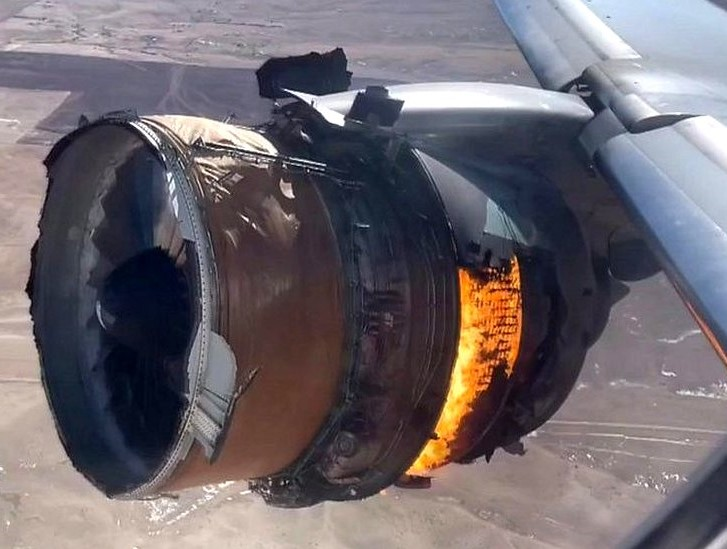
\includegraphics[scale=0.3]{turbine_failure.jpg}
                        \caption{Turbine failure mid-flight \cite{bbc-news-2021}}
                    \end{figure}
                \end{column}
            \end{columns}
        \end{frame}


        \begin{frame}{Introduction}{Problem Statement}

            Predictive maintenance faces 2 main challenges:
            \begin{block}{Implementation}
                Need a model to estimate the RUL of a set of machinery, in an efficient and reliable manner
            \end{block}

            \begin{alertblock}{Interpretability}
                Need to \textit{understand} why a model produces a given RUL estimate, becomes more important in critical environments
            \end{alertblock}

        \end{frame}

    \section{Objectives}

        \begin{frame}
            \frametitle{Objectives}
            \begin{columns}
                \begin{column}{0.45\textwidth}
                    This research project aims to develop:
                    \begin{enumerate}
                        \item PdM framework to predict RUL for a designated fleet of machinery
                        \item Model which ensures reproducibility, stability, robustness and confidence
                        \item Tools to interpret and visualize the model's predictions
                    \end{enumerate}
                \end{column}
                \begin{column}{0.55\textwidth}
                    \begin{figure}[!htbp]
                        \centering
                        \includegraphics[scale=0.04]{uniform_fleet.jpg}
                        \caption{Sample of a uniform fleet of cars}
                    \end{figure}
                \end{column}
            \end{columns}
        \end{frame}

        \begin{frame}{Objectives}{Scope}
            \begin{columns}
                \begin{column}{0.5\textwidth}
                    The previous objectives are to be accomplished subject to the following constraints and assumptions:
                    \begin{itemize}
                        \item RUL prediction of an uniform fleet of machines
                        \item Availability of a labeled dataset with run to failure sequences of each machine
                    \end{itemize}
                \end{column}
                \begin{column}{0.5\textwidth}
                    \begin{figure}[!htbp]
                        \centering
                        \includegraphics[scale=0.4]{machine_efficiency.png}
                        \caption{Efficiency loss as a machine operates}
                    \end{figure}
                \end{column}
            \end{columns}
        \end{frame}

        \begin{frame}{Objectives}{Loss Function}
            The 2021 PHMAP challenge proposed the loss function \eqref{eqn:phmap_loss}; the average of the RMSE and NASA's scoring function \cite{saxena2008damage}.
            \begin{equation} \label{eqn:phmap_loss}
                \begin{gathered}
                    \mathcal{L}(y, \hat{y}) = \frac{1}{2} \left(\sqrt{\frac{1}{m}\sum_{i=1}^{m} (y_i - \hat{y}_i)^{2}} + \frac{1}{m}\sum_{i=1}^{m} \exp (\alpha \cdot (y_i - \hat{y}_i)) - 1 \right) \\
                    \alpha = \begin{cases}
                        \frac{-1}{10} & \text{if } y_i - \hat{y}_i \leq 0 \\
                        \frac{1}{13} & \text{if } y_i - \hat{y}_i > 0
                    \end{cases}
                \end{gathered}
            \end{equation}

            As a remark, \eqref{eqn:phmap_loss} is an asymmetric loss function with a higher penalty for overestimates.
        \end{frame}

    \section{Exploratory Data Analysis}

        \begin{frame}{Exploratory Data Analysis}{NCMAPSS Dataset}

            Flight conditions and readings from a fleet of turbofan engines,
            derived from NASA's CMAPSS model, including real flight conditions and relates the degradation process to the operating history of the machine. \cite{arias2021aircraft}
            \begin{itemize}
                \item Used in the PHMAP 2021 Data Challenge \cite{phm-conference}
                \item State of the art prognosis dataset (akin to MNIST and CIFAR for CV)
            \end{itemize}

            \begin{figure}[!htbp]
                \centering
                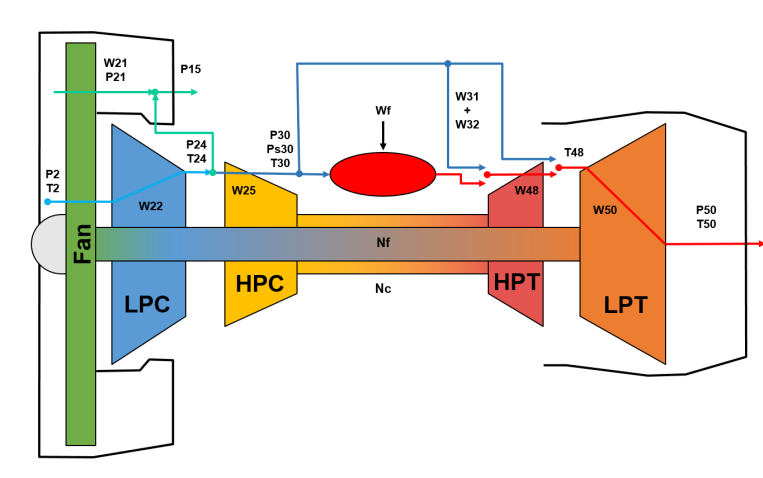
\includegraphics[scale=0.35]{cmapss_turbofan.png}
                \caption{CMAPSS turbofan engine schematic}
            \end{figure}
        \end{frame}

        \begin{frame}{Exploratory Data Analysis}{Data Overview}
            \begin{columns}
                \begin{column}{0.4\textwidth}
                    \begin{itemize}
                        \item Split into 10 h5 files
                        \item Sampling frequency of 1 second
                        \item Contains sensor readings, environmental descriptors, auxiliary variables, virtual sensor readings and RUL values
                        \item Corrupted file in the dataset
                    \end{itemize}
                \end{column}
                \begin{column}{0.6\textwidth}
                    \begin{table}[!htbp]
                        \centering
                        \scalebox{0.5}{
                        \begin{tabular}{ |l|l|l| }
                            \hline
                            Symbol & Description & Units \\
                            \hline
                            alt & Altitude & ft \\
                            Mach & Flight Mach number & - \\
                            TRA & Throttle-resolver angle & \% \\
                            T2 & Total temperature at fan inlet & °R \\
                            \hline
                            Wf & Fuel flow & pps \\
                            Nf & Physical fan speed & rpm \\
                            Nc & Physical core speed & rpm \\
                            T24 & Total temperature at LPC outlet & °R \\
                            T30 & Total temperature at HPC outlet & °R \\
                            T48 & Total temperature at HPT outlet & °R \\
                            T50 & Total temperature at LPT outlet & °R \\
                            P15 & Total pressure in bypass-duct & psia \\
                            P2 & Total pressure at fan inlet & psia \\
                            P21 & Total pressure at fan outlet & psia \\
                            P24 & Total pressure at LPC outlet & psia \\
                            Ps30 & Static pressure at HPC outlet & psia \\
                            P40 & Total pressure at burner outlet & psia \\
                            P50 & Total pressure at LPT outlet & psia \\
                            \hline
                            RUL & Remaining Useful Life & cycles \\
                            \hline
                            unit & Unit number & - \\
                            cycle & Flight cycle number & - \\
                            Fc & Flight class & - \\
                            hs & Health state & - \\
                            \hline
                        \end{tabular}}
                        \label{tab:dataset_info}
                        \caption{General description of dataset variables  \cite{phm-conference}}
                    \end{table}
                \end{column}
            \end{columns}

        \end{frame}

        \begin{frame}{Exploratory Data Analysis}{Flight Class Distribution}
            \begin{figure}[!htbp]
                \centering
                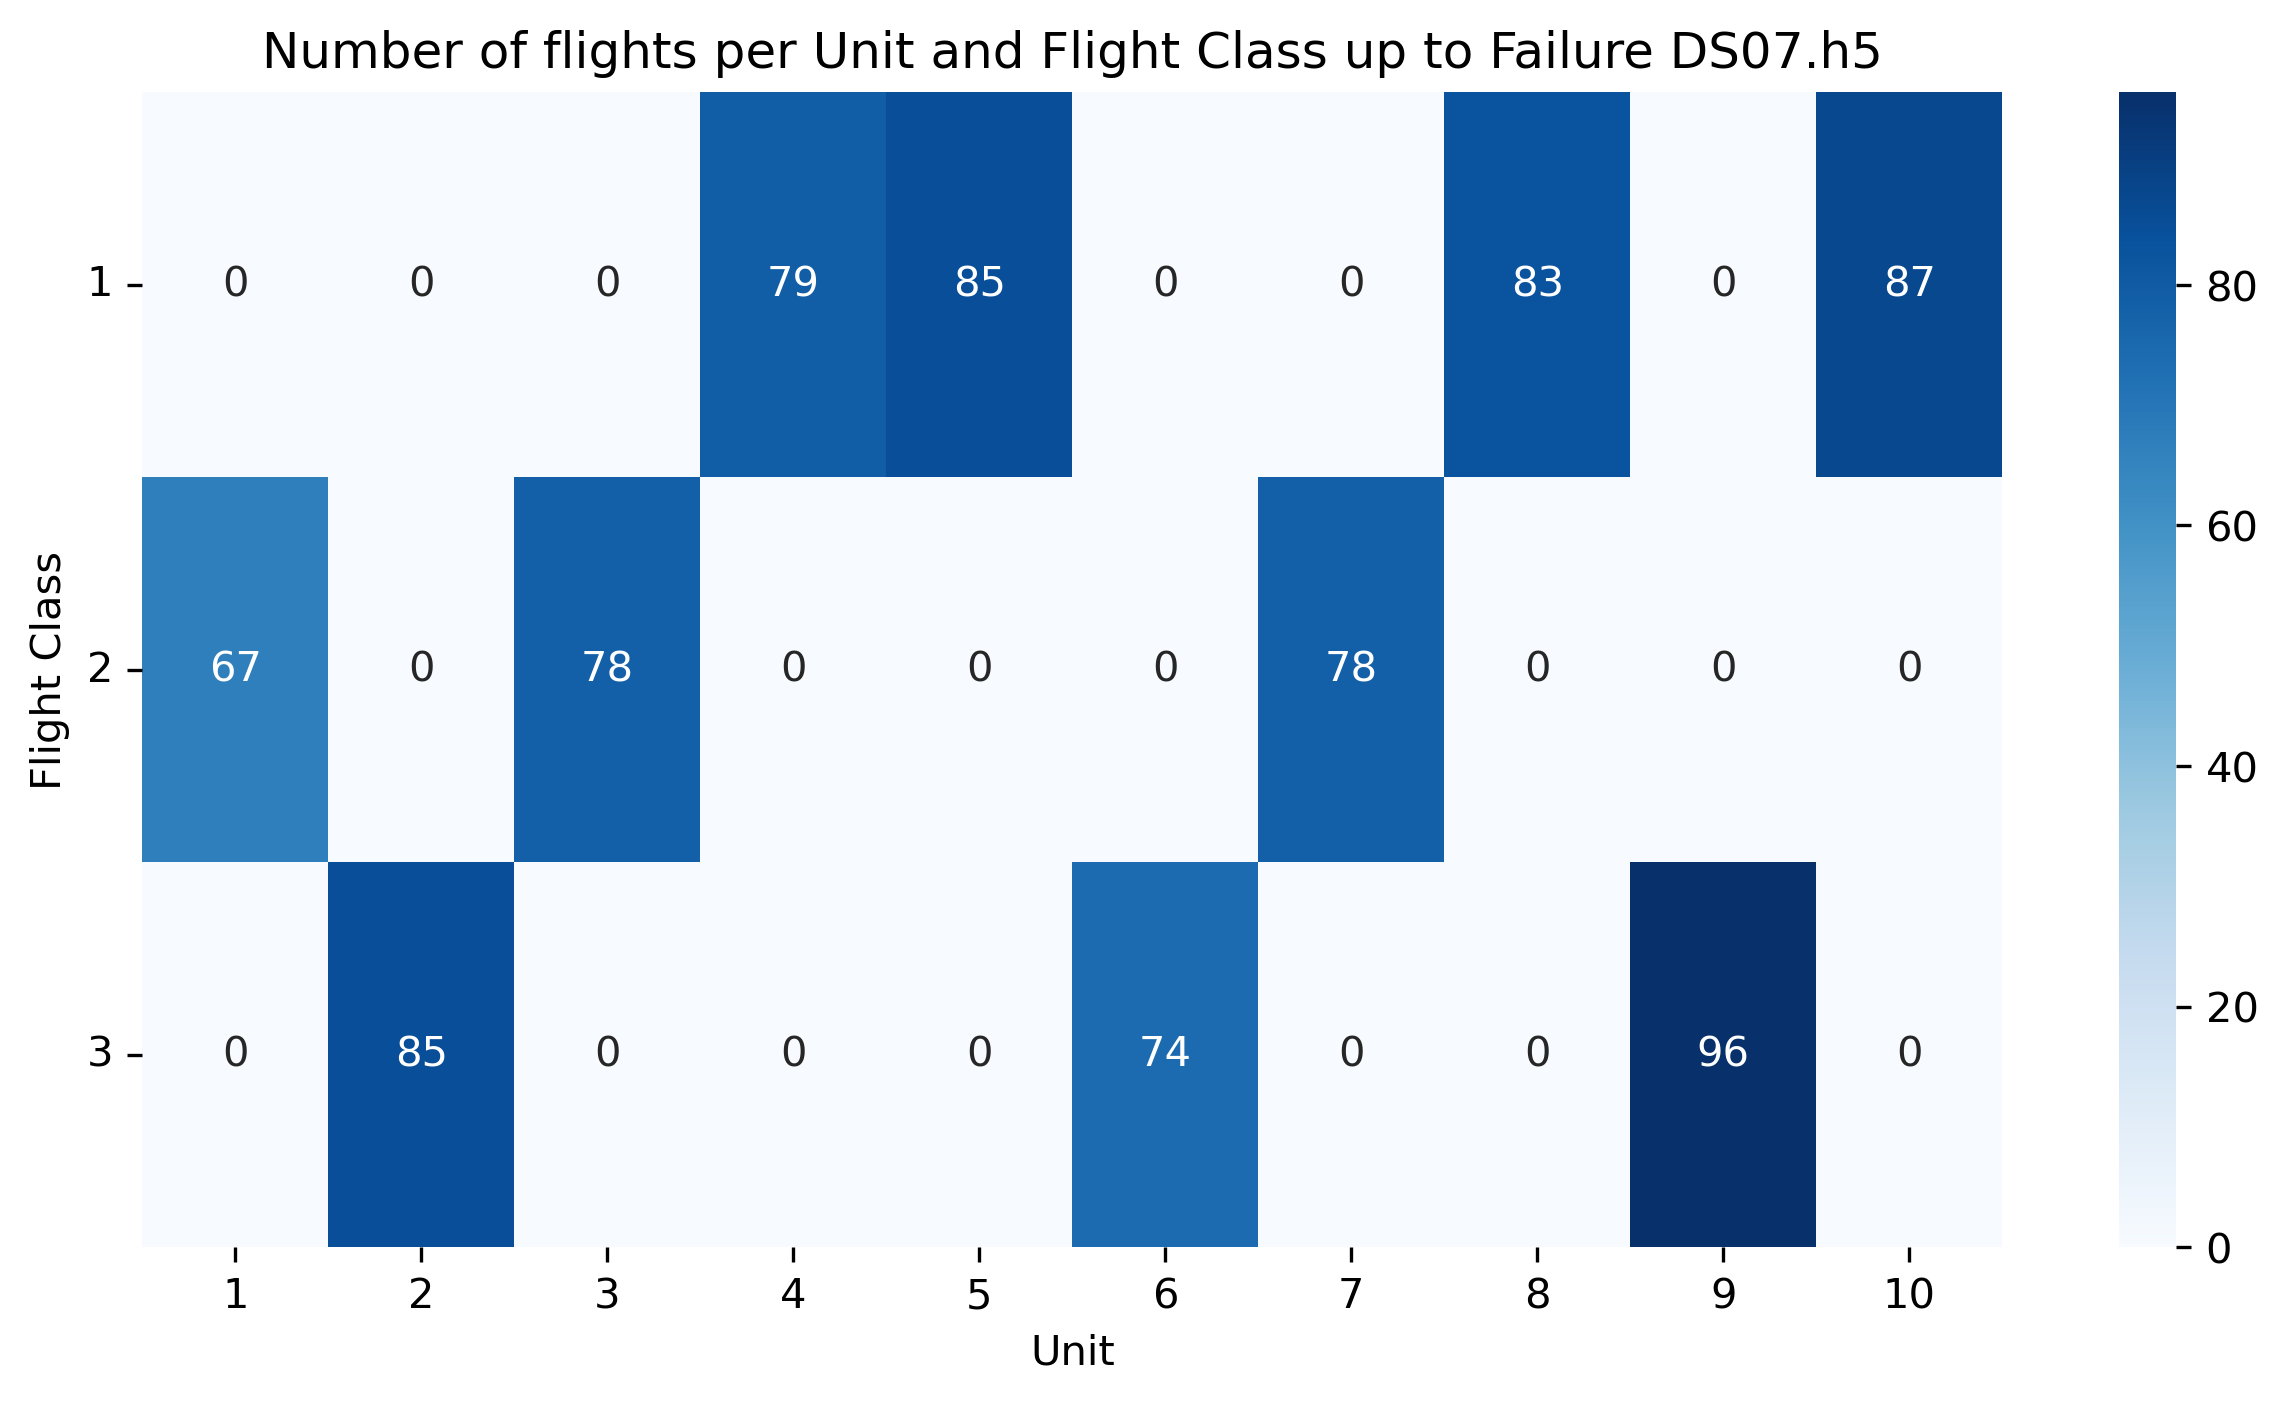
\includegraphics[scale=0.4]{fligt_class_per_unit_DS07.h5.png}
                \caption{Flights recorded for each class per unit}
            \end{figure}
            Flight classes encode flight duration\footnotemark[1], and there are no inter-class units
            \footnotetext[1]{FC1 ranges between 1 and 3 hours, FC2 between 3 and 5, and FC3 is greater than 5}
        \end{frame}

        \begin{frame}{Exploratory Data Analysis}{Sample Operating Conditions}
            \begin{figure}[!htbp]
                \centering
                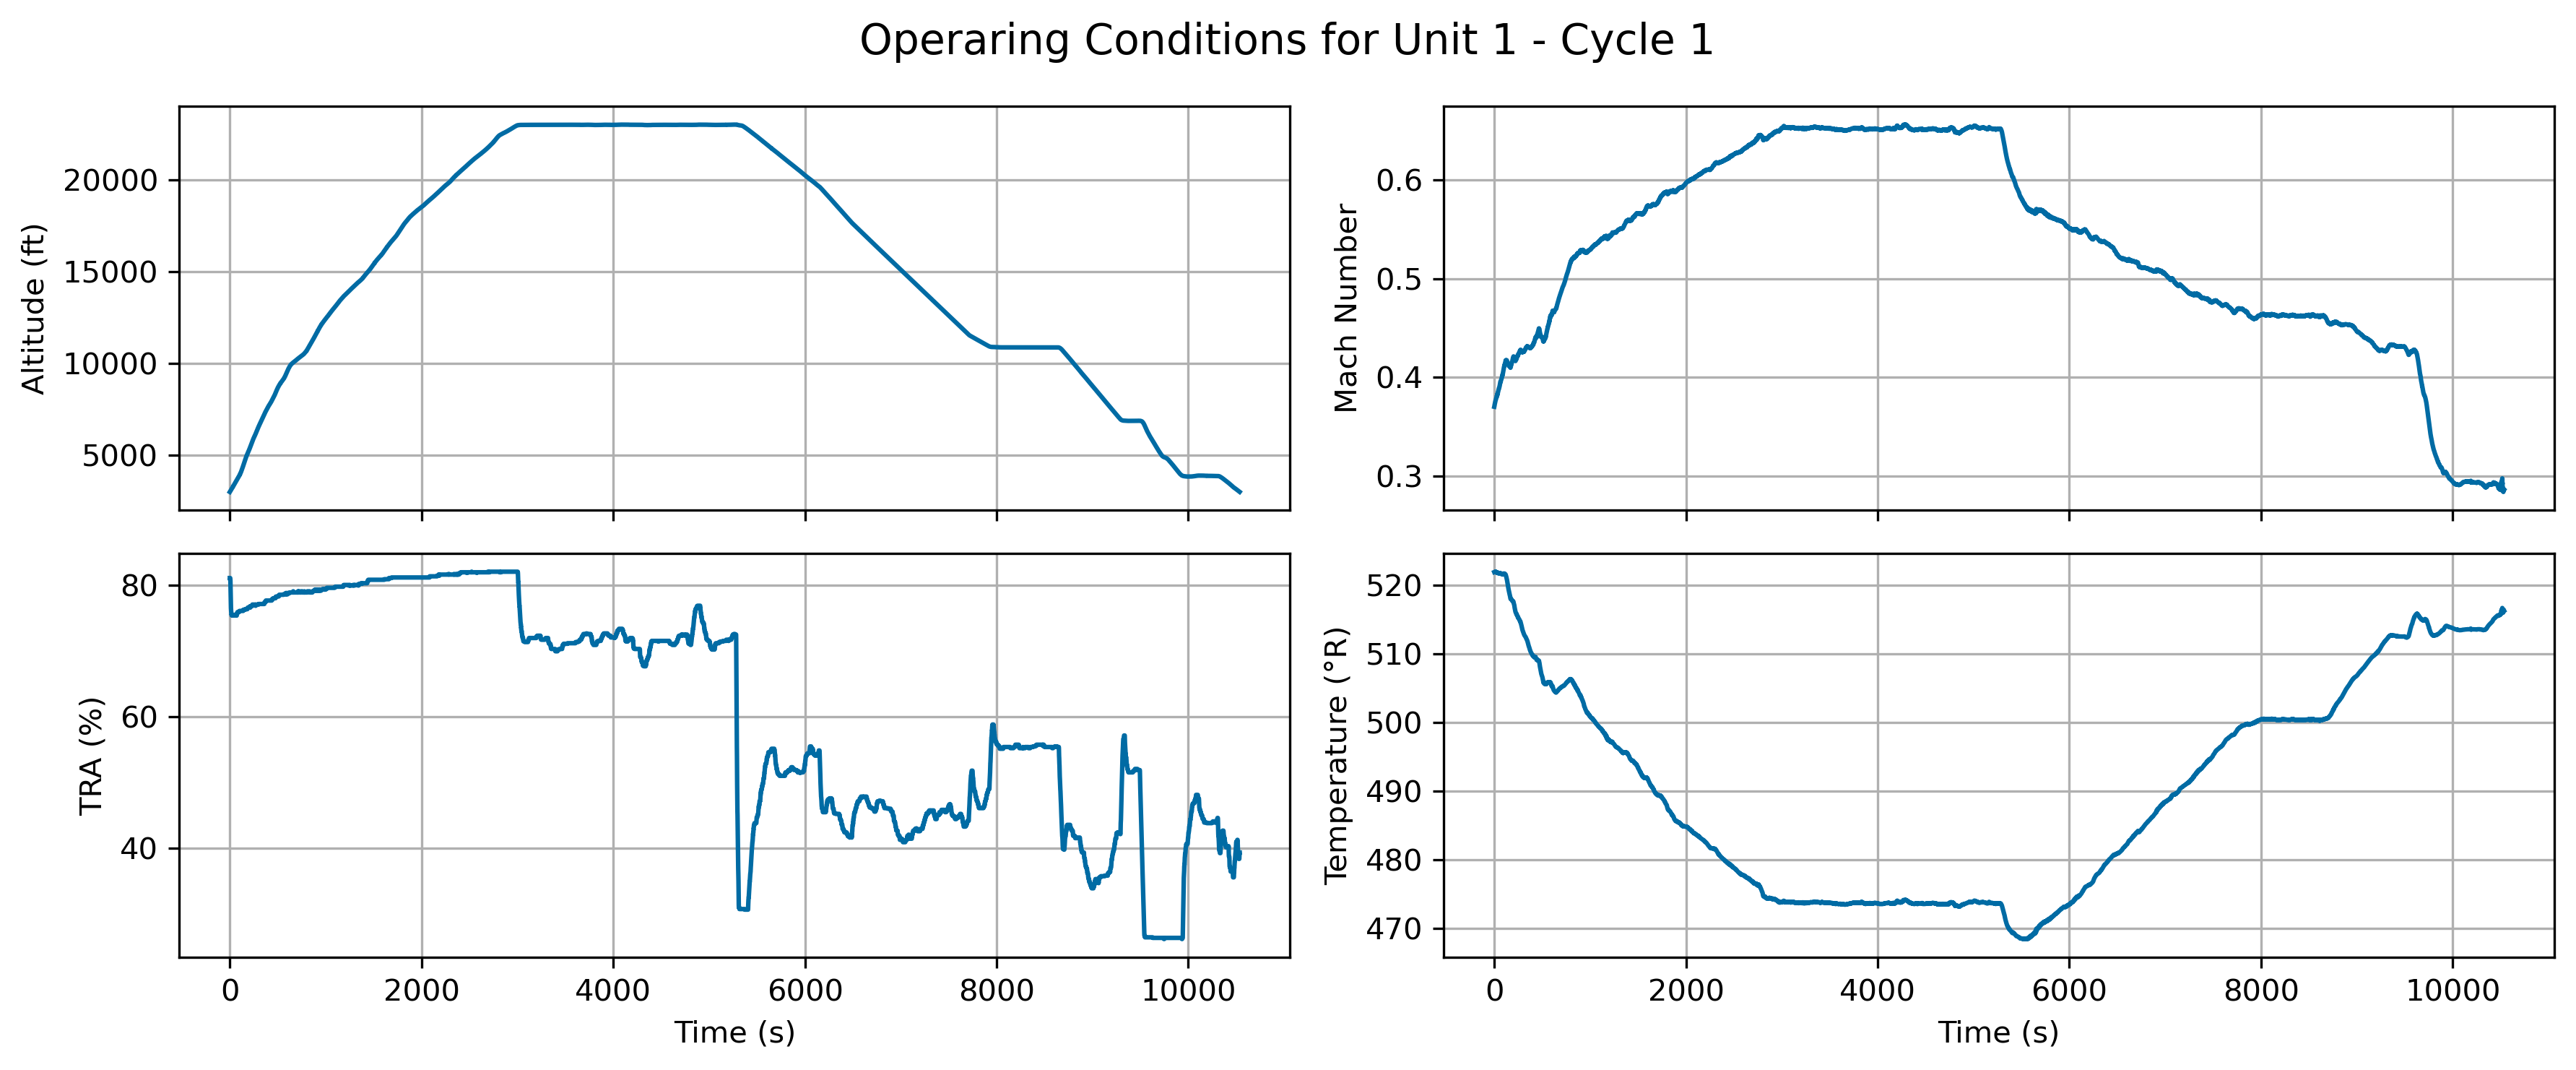
\includegraphics[scale=0.35]{operating_conditions_unit_1_cycle_1.png}
                \caption{Operating conditions for the first flight of Unit 1}
            \end{figure}
        \end{frame}

        \begin{frame}{Exploratory Data Analysis}{Operating Conditions per Flight Class}
            \begin{figure}[!htbp]
                \centering
                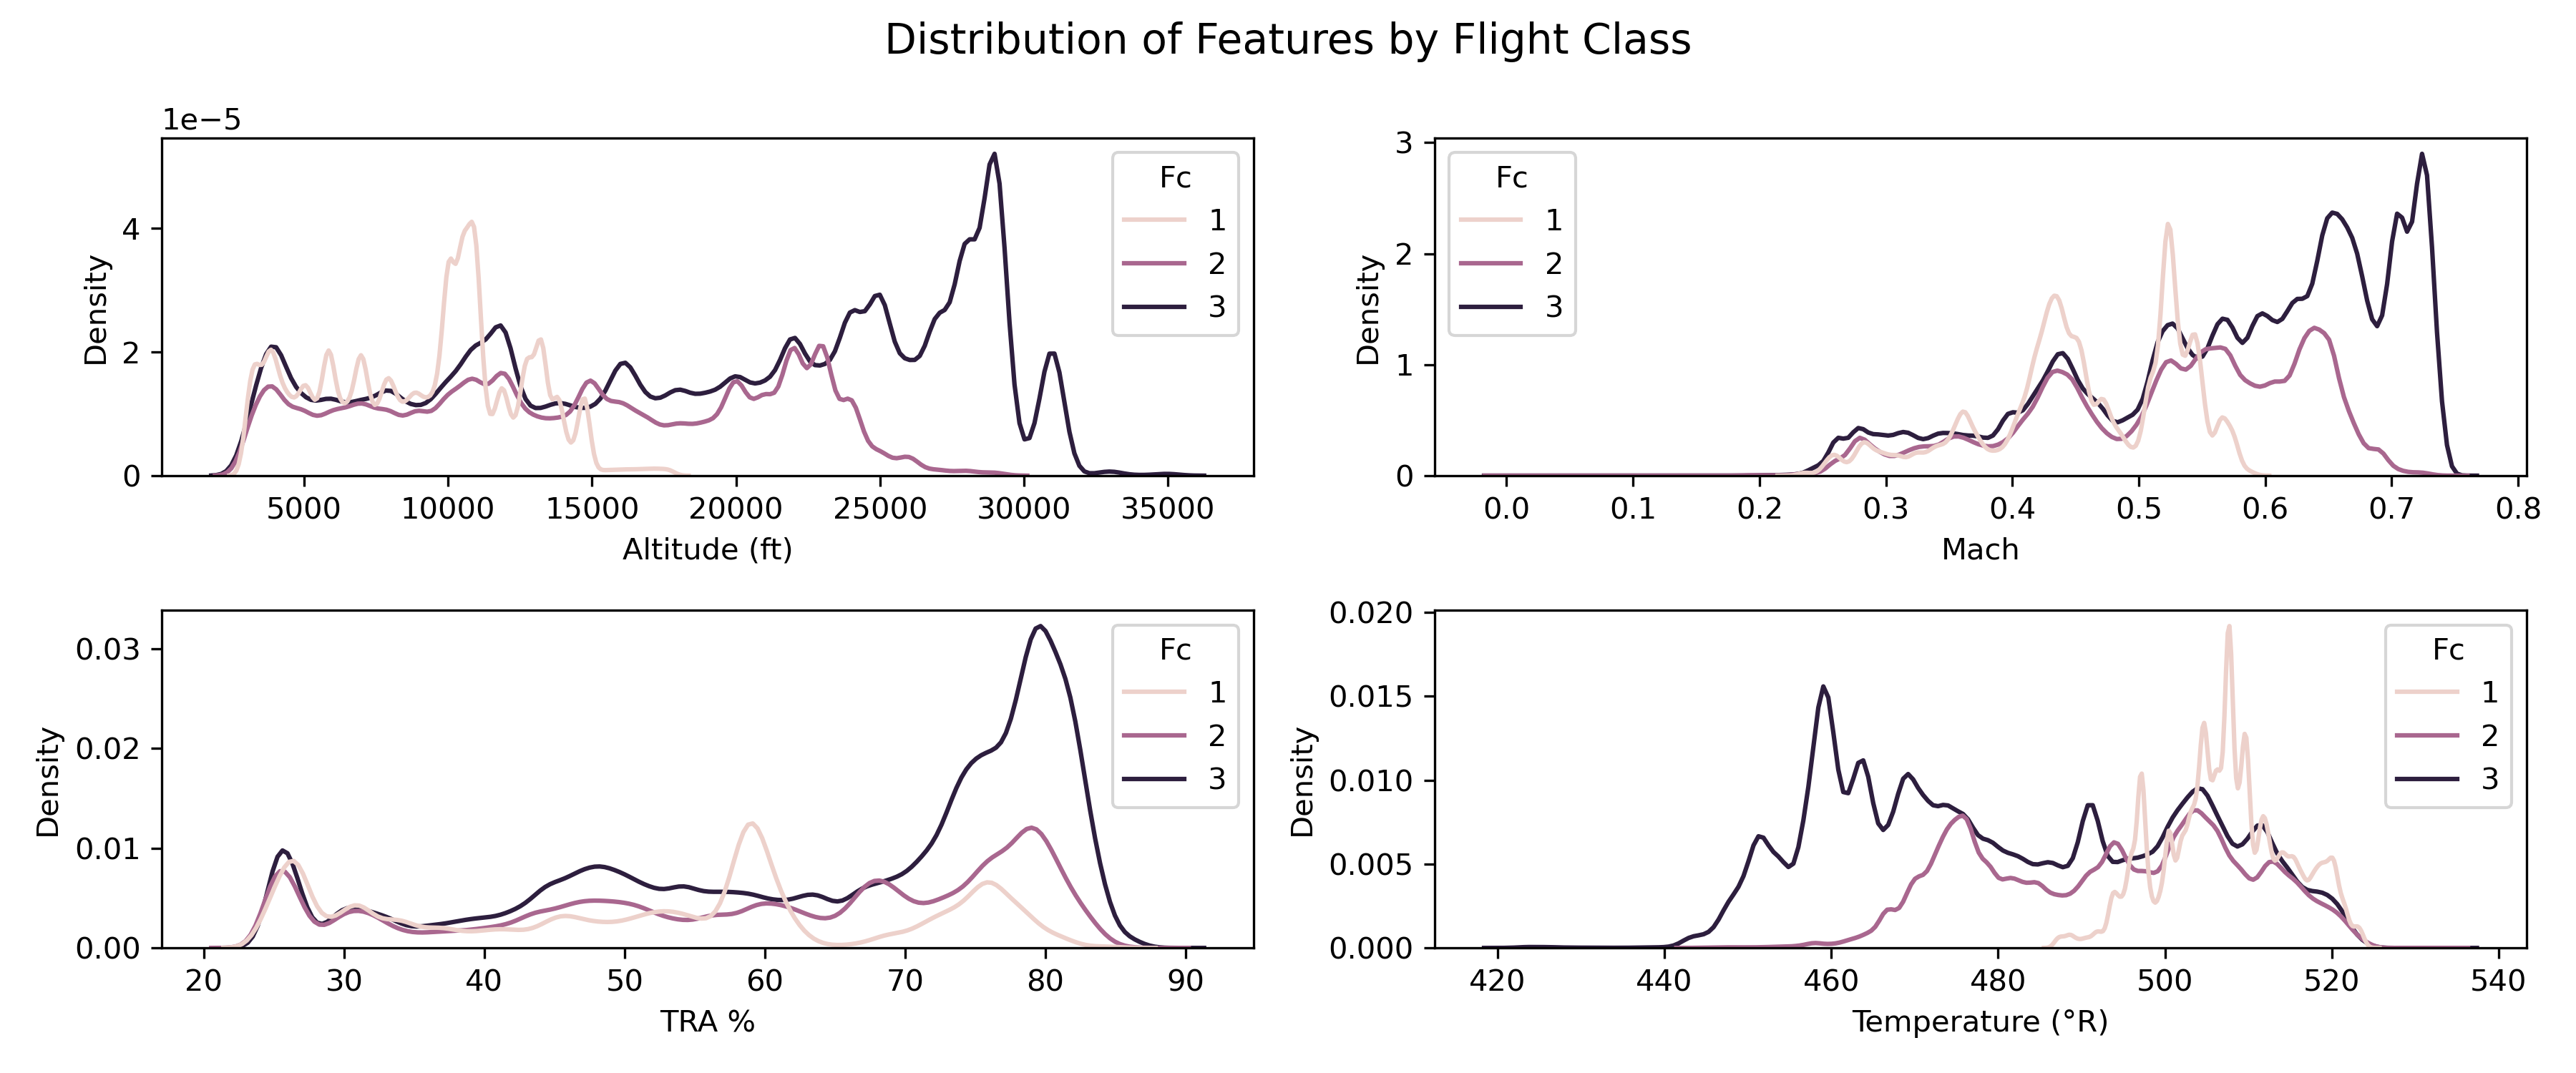
\includegraphics[scale=0.35]{features_per_condition_fc.png}
                \caption{Distribution of operating conditions per Flight Class}
            \end{figure}

            Distinctive operating conditions per FC where FC2 can be seen as a mixture of FC1 and FC3
        \end{frame}

        \begin{frame}{Exploratory Data Analysis}{Final Sensor Readings}
            \begin{figure}[!htbp]
                \centering
                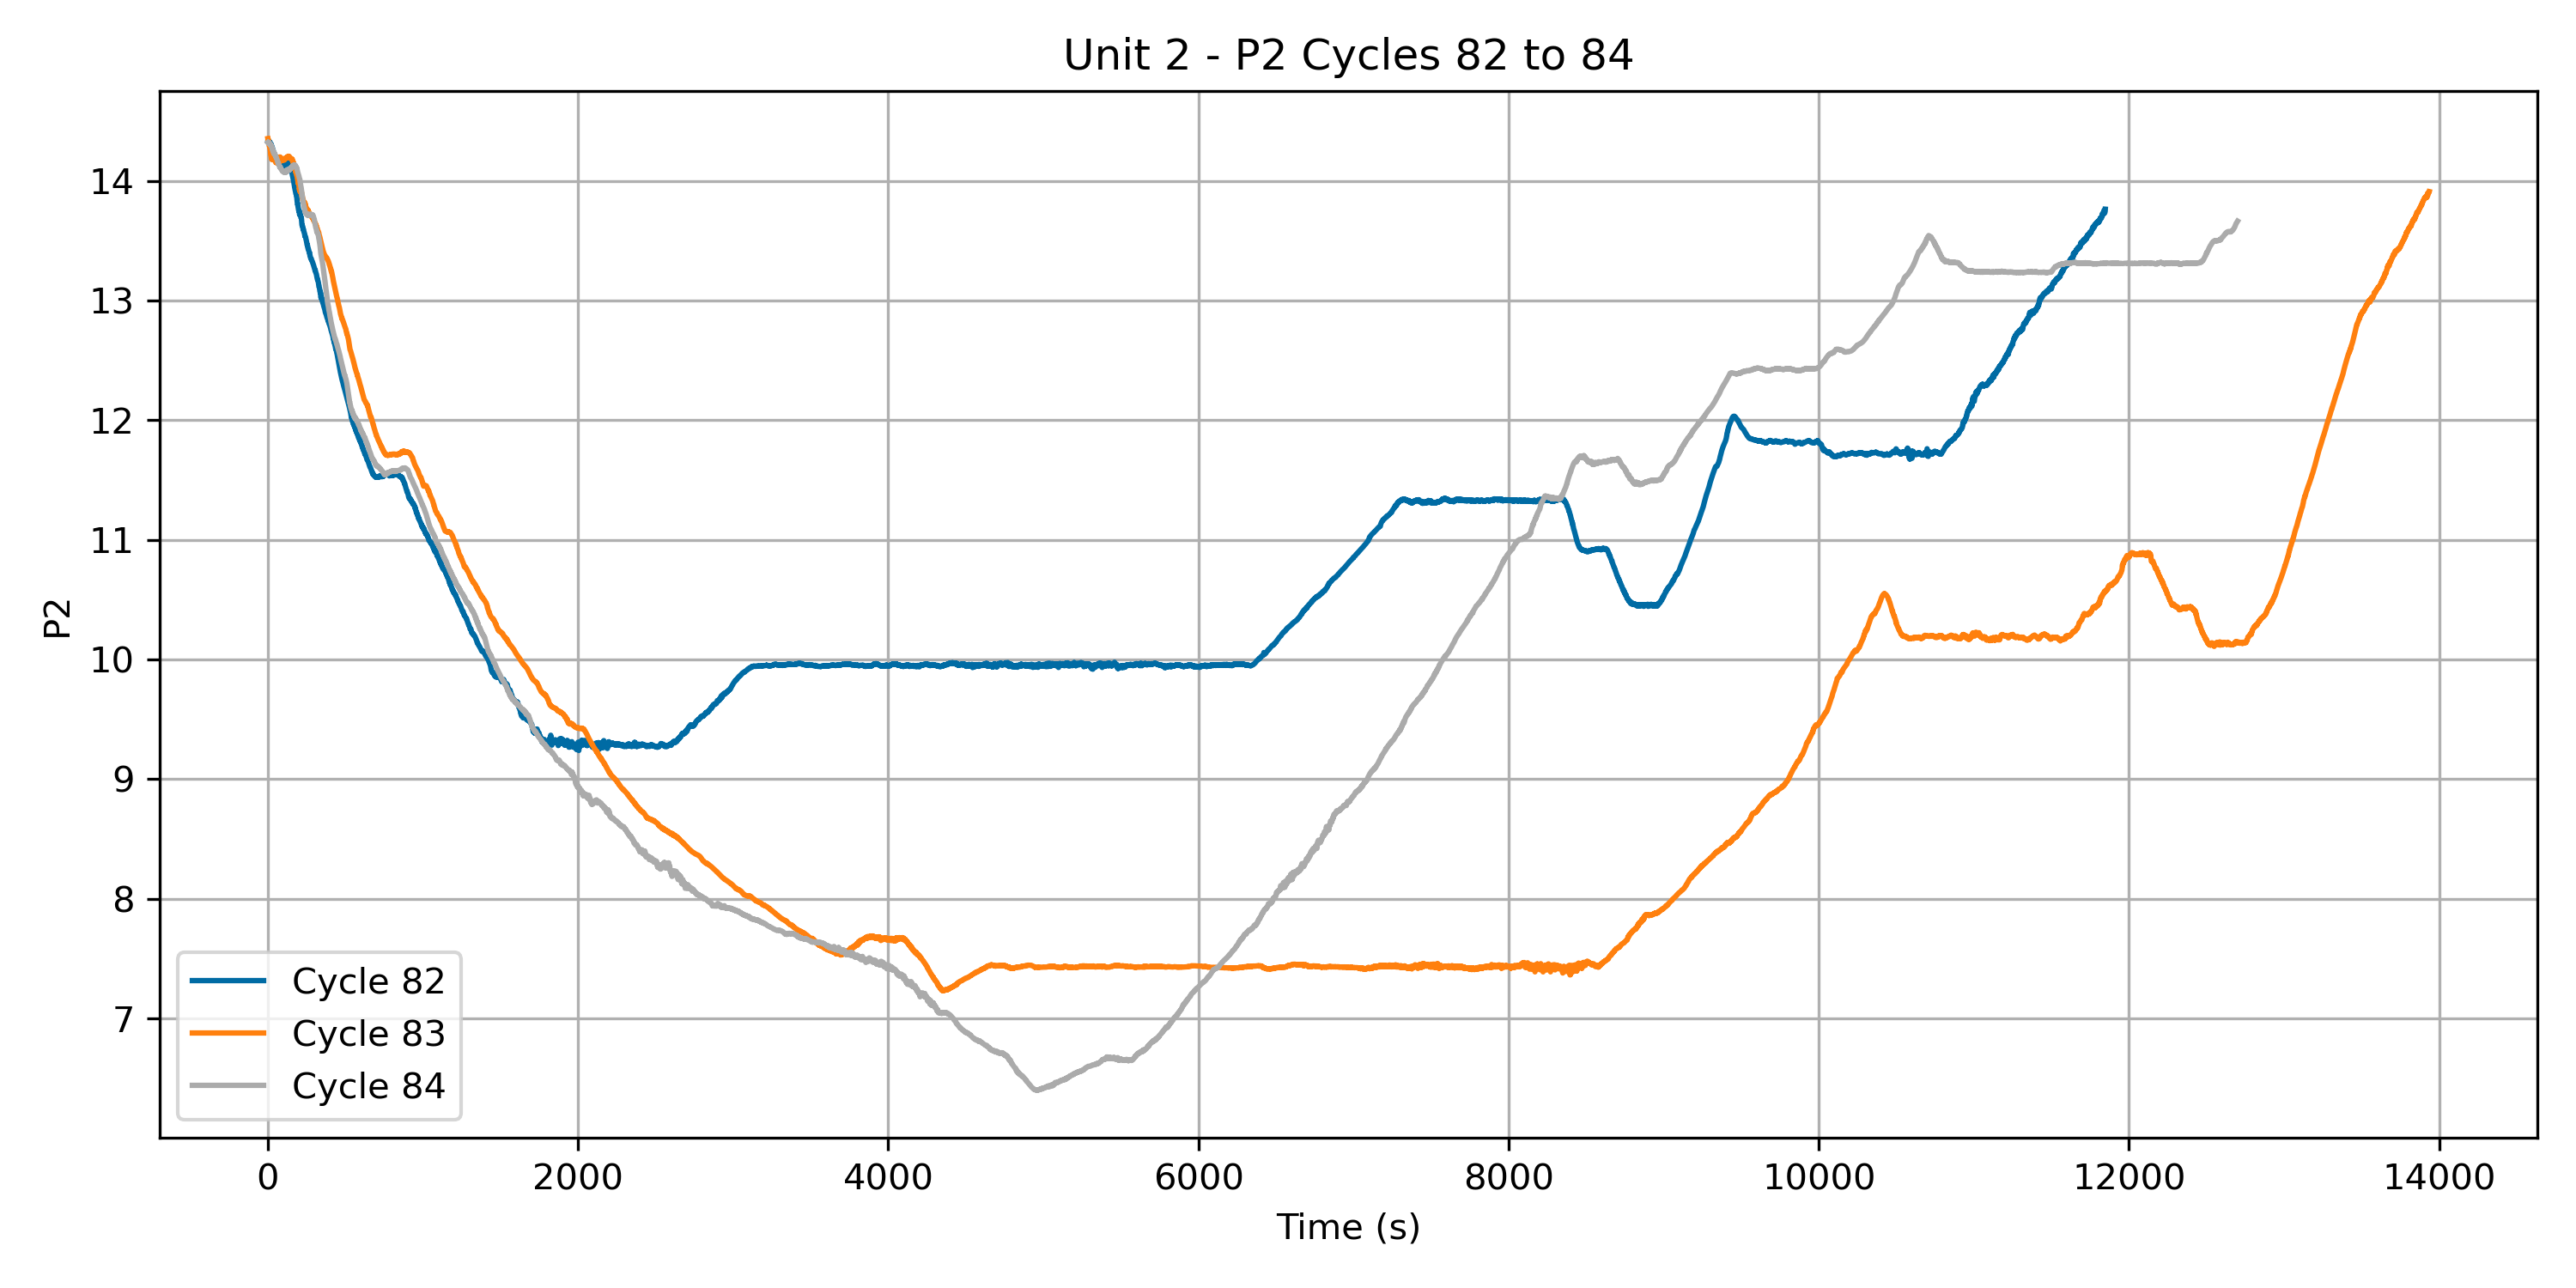
\includegraphics[scale=0.35]{unit_2_P2_cycles_82_84.png}
                \caption{Total Pressure at fan inlet (P2) for the last 3 cycles of unit 2}
            \end{figure}
            Smoothness degradation with a presence of new plateaus near the end of the flight
        \end{frame}

    \section{Methodology}

        \begin{frame}{Methodology}{Proposed Methodology}
            \begin{figure}[!htbp]
                \centering
                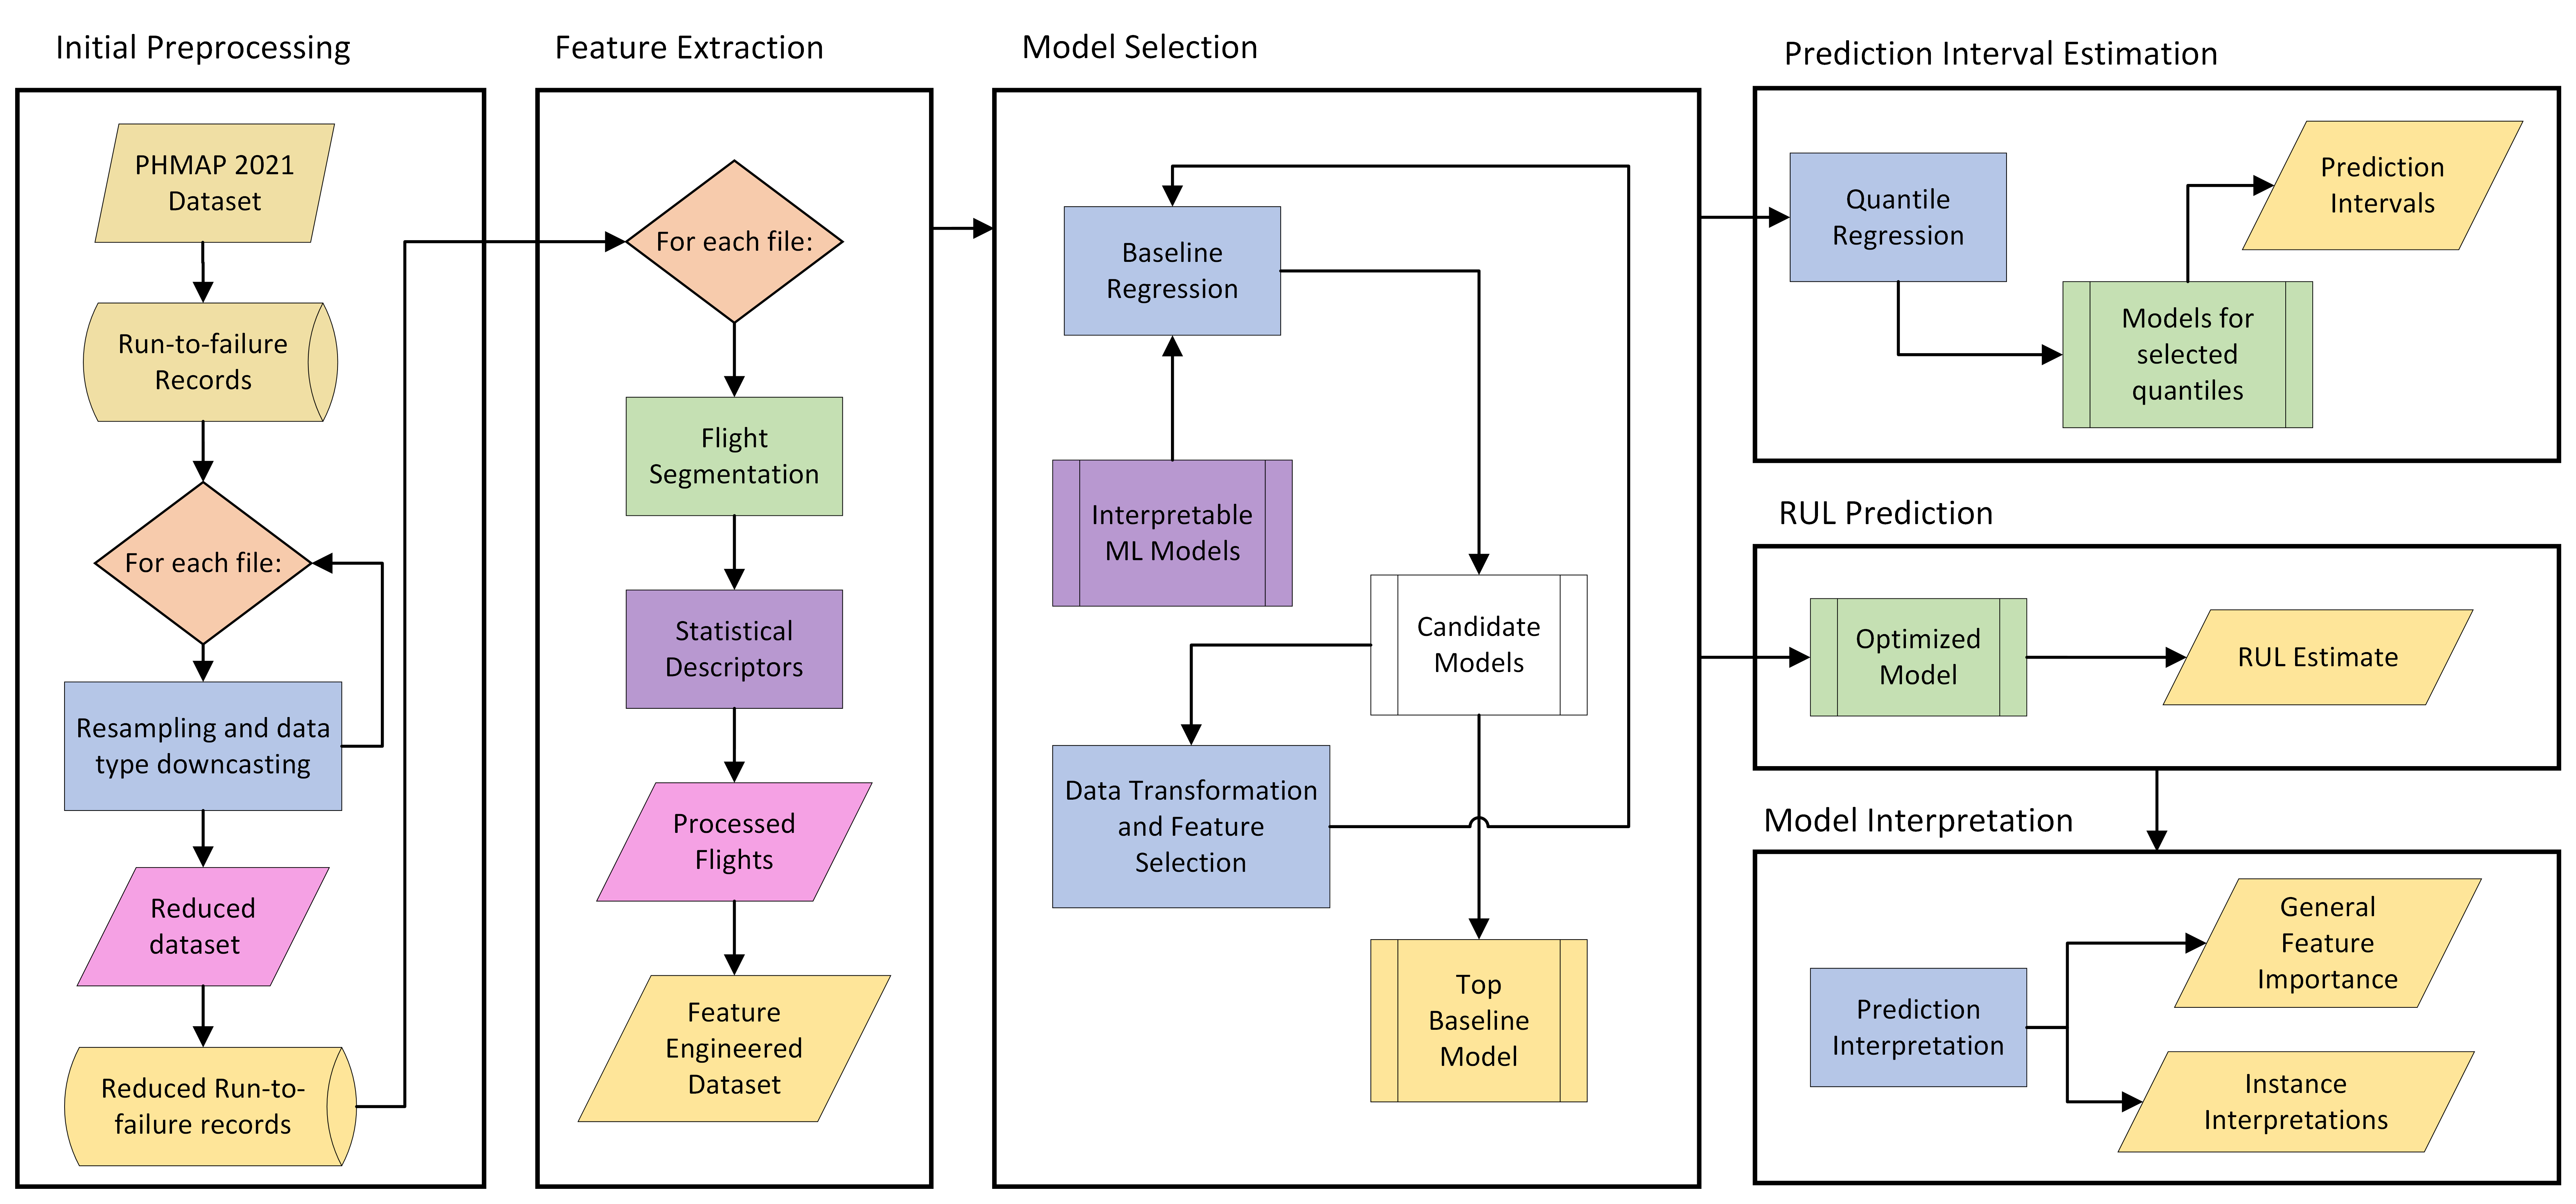
\includegraphics[scale=0.2]{research_diagram.png}
                \caption{Proposed Methodology}
            \end{figure}
        \end{frame}

        \subsection{Data Resampling and Downcasting}

            \begin{frame}{Data Resampling and Downcasting}
                \begin{columns}
                    \begin{column}{0.45\textwidth}
                        Sensor readings every second can lead to large arrays, think about sampling frequency (1 Hz, 1 KHz, 1 MHz, etc\dots) and data types.
                        \begin{itemize}
                            \item Resampling to catch the general shape
                            \item Downcasting to a datatype with lower memory footprint (64bit float to 32bit float)
                        \end{itemize}
                    \end{column}
                    \begin{column}{0.5\textwidth}
                        \begin{figure}[!htbp]
                            \centering
                            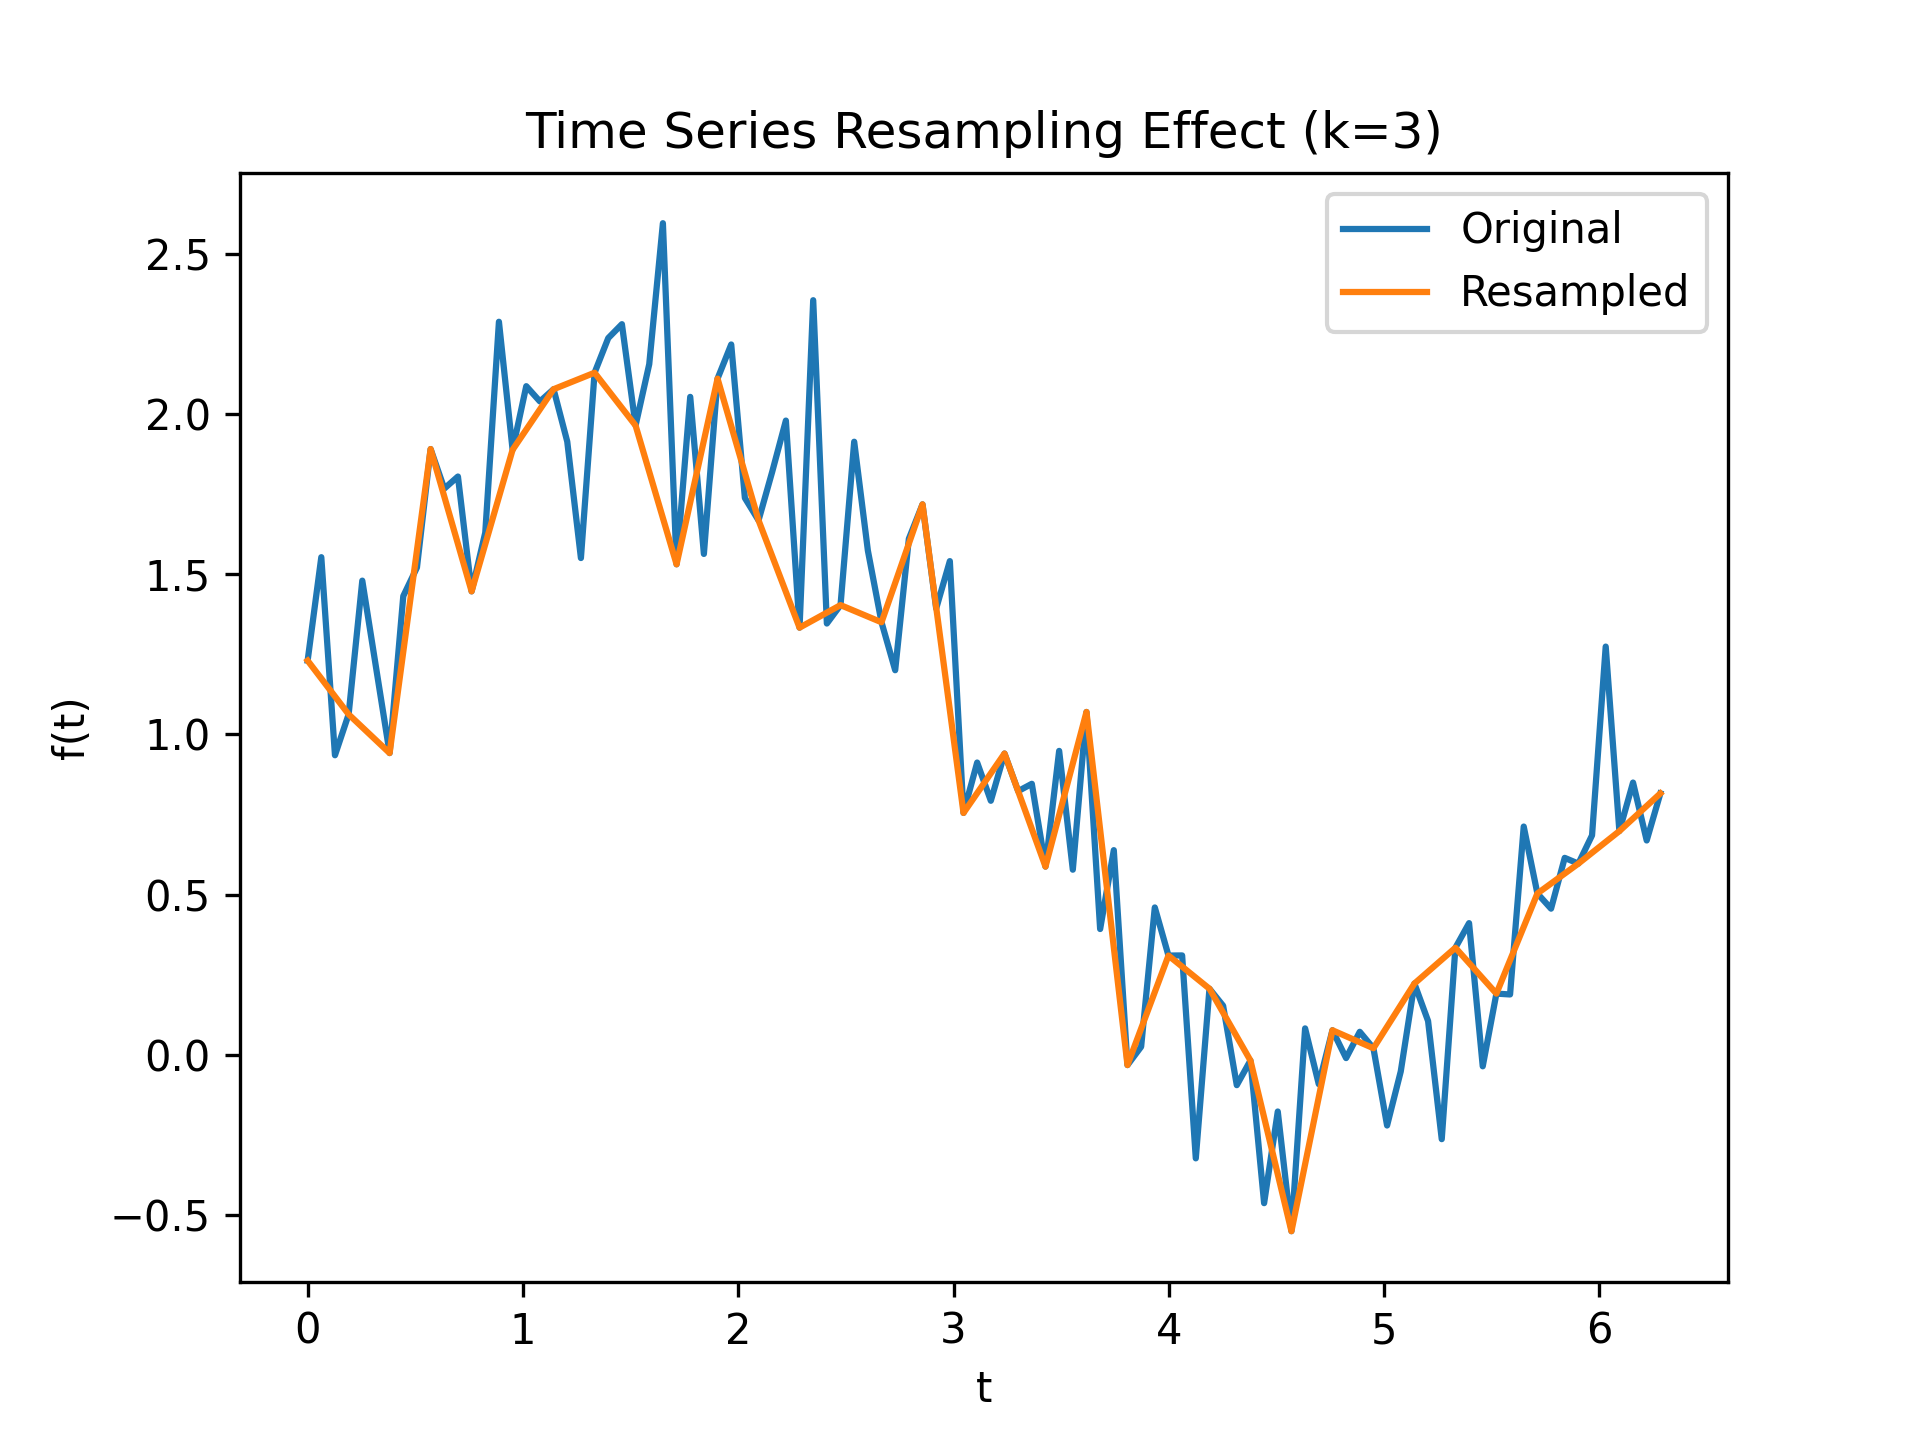
\includegraphics[scale=0.4]{resampling_series.png}
                            \caption{Time Series Resampling and Downcasting Effect}
                        \end{figure}
                    \end{column}
                \end{columns}
            \end{frame}

        \subsection{Time Series Segmentation}

            \begin{frame}{Time Series Segmentation}

                \begin{alertblock}{Problem}
                    Dataset consists of a set of multivariate time series of varying length with a distinct number of events per series
                \end{alertblock}
                \begin{figure}[!htbp]
                    \centering
                    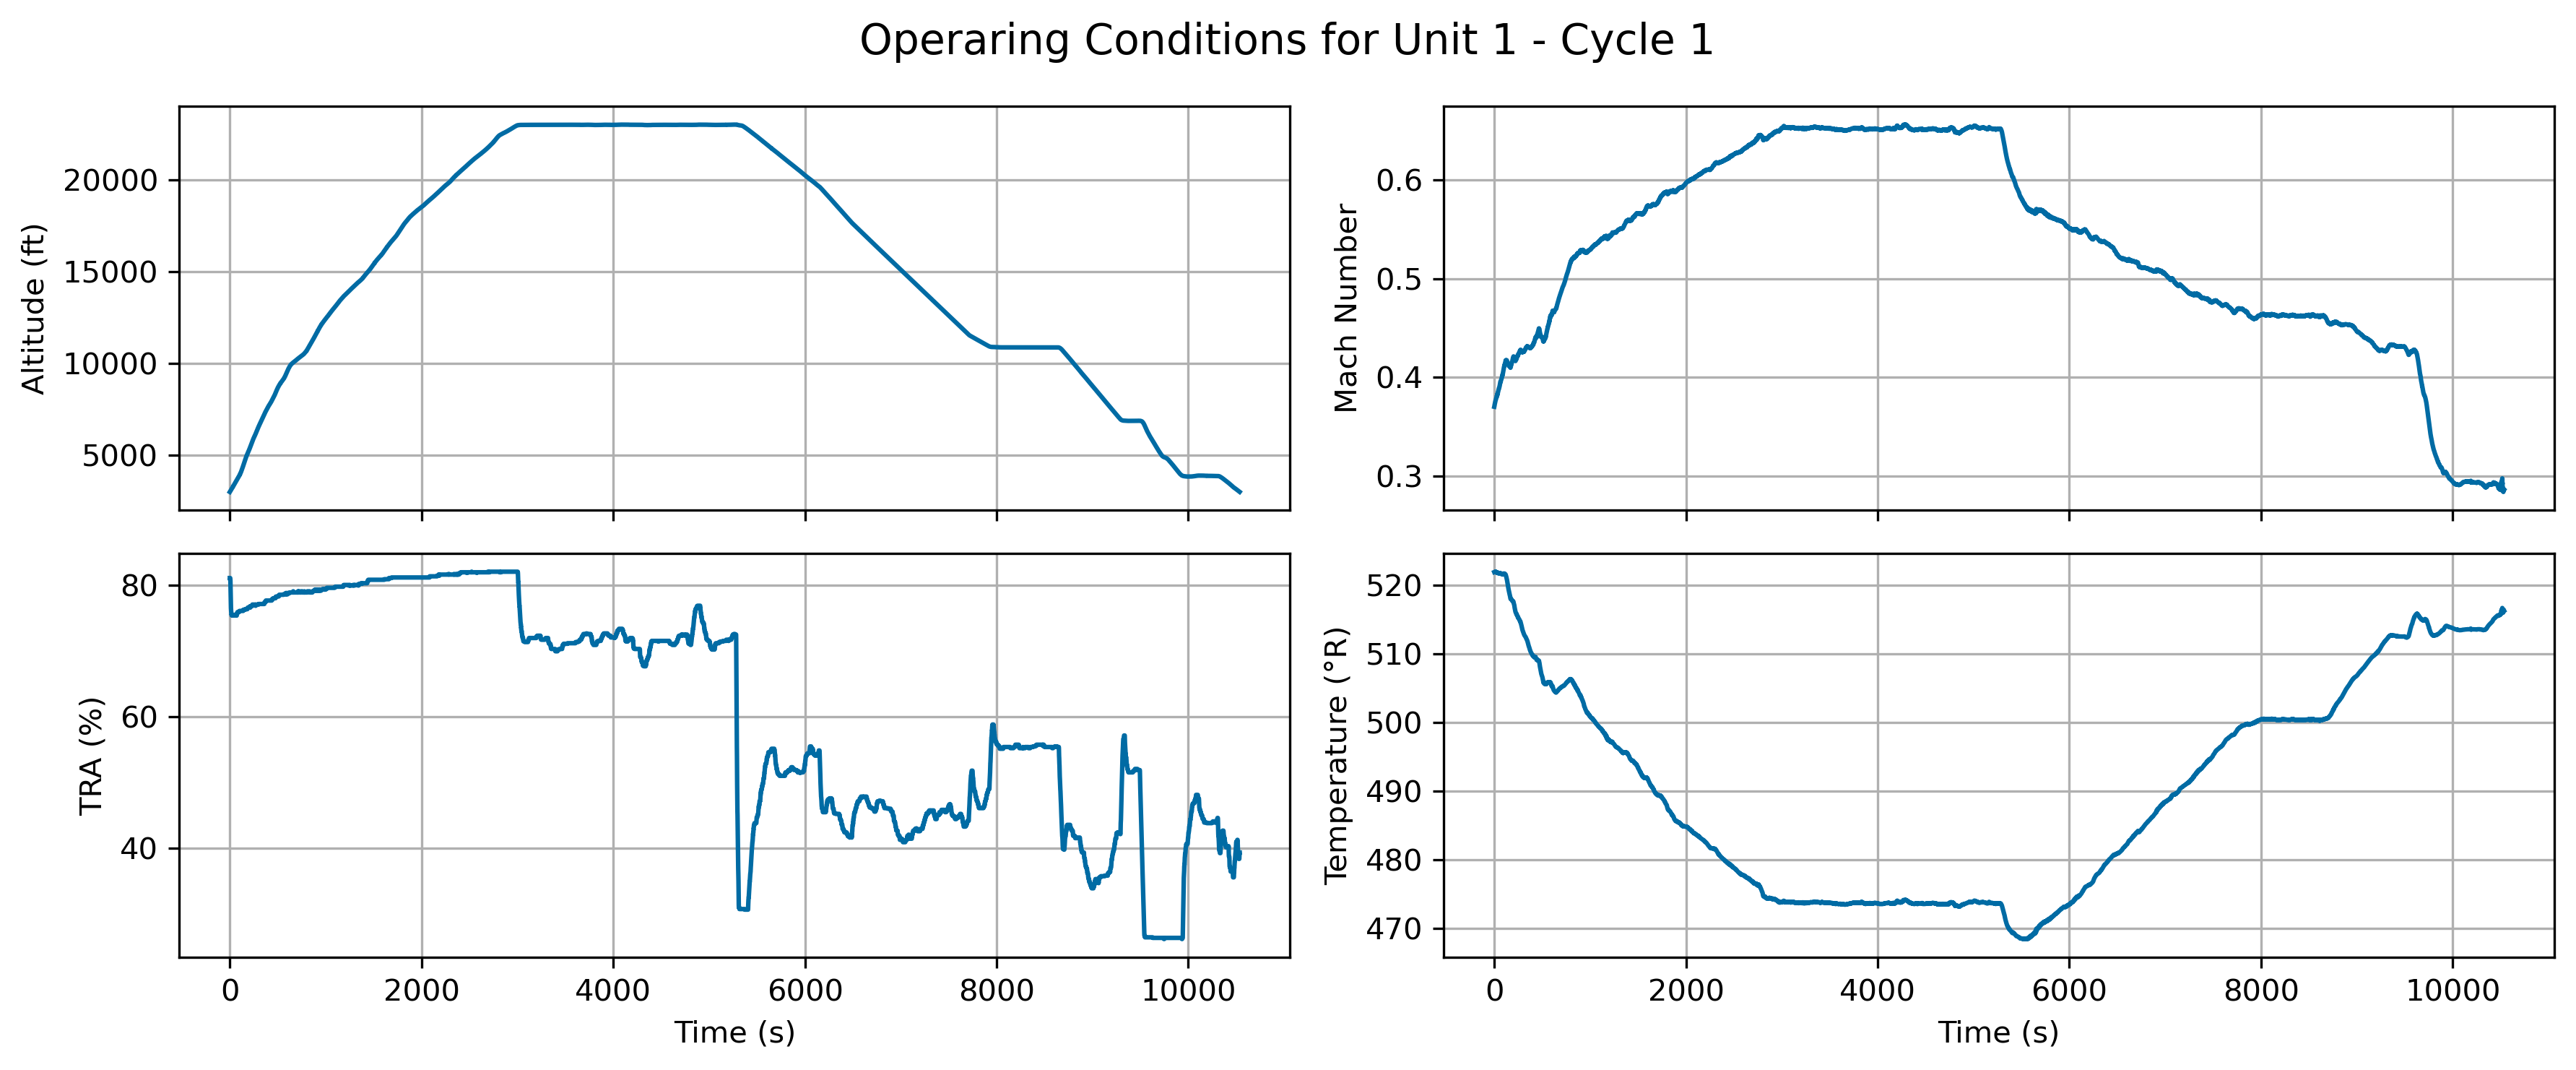
\includegraphics[scale=0.3]{operating_conditions_unit_1_cycle_1.png}
                    \caption{Operating conditions of Plane 1 during its first flight}
                \end{figure}

                \note[item]{Altitude almost always seems to have 3 states, ascent, plateau, descent}
                \note[item]{Mechanical operations vary throughout the flight, there's no smooth increase or decrease, rather multiple operating stages}
                \note[item]{Take advantage of the syncrhonization between time series, look at plateau}
            \end{frame}

            \begin{frame}{Time Series Segmentation}{Basics}
                For a given signal $Y = \{\boldsymbol{y}_t\}_{t=1}^{t=T}$ of $T$ samples, where $y_t \in \mathbb{R}^d$, we assume there exists a set $\mathcal{T} = \{t_{1}^{*}, t_{2}^{*}, \dots, t_{n}^{*}\}$ coding the $n-1$ stages of $Y$

                \begin{figure}[!htbp]
                    \centering
                    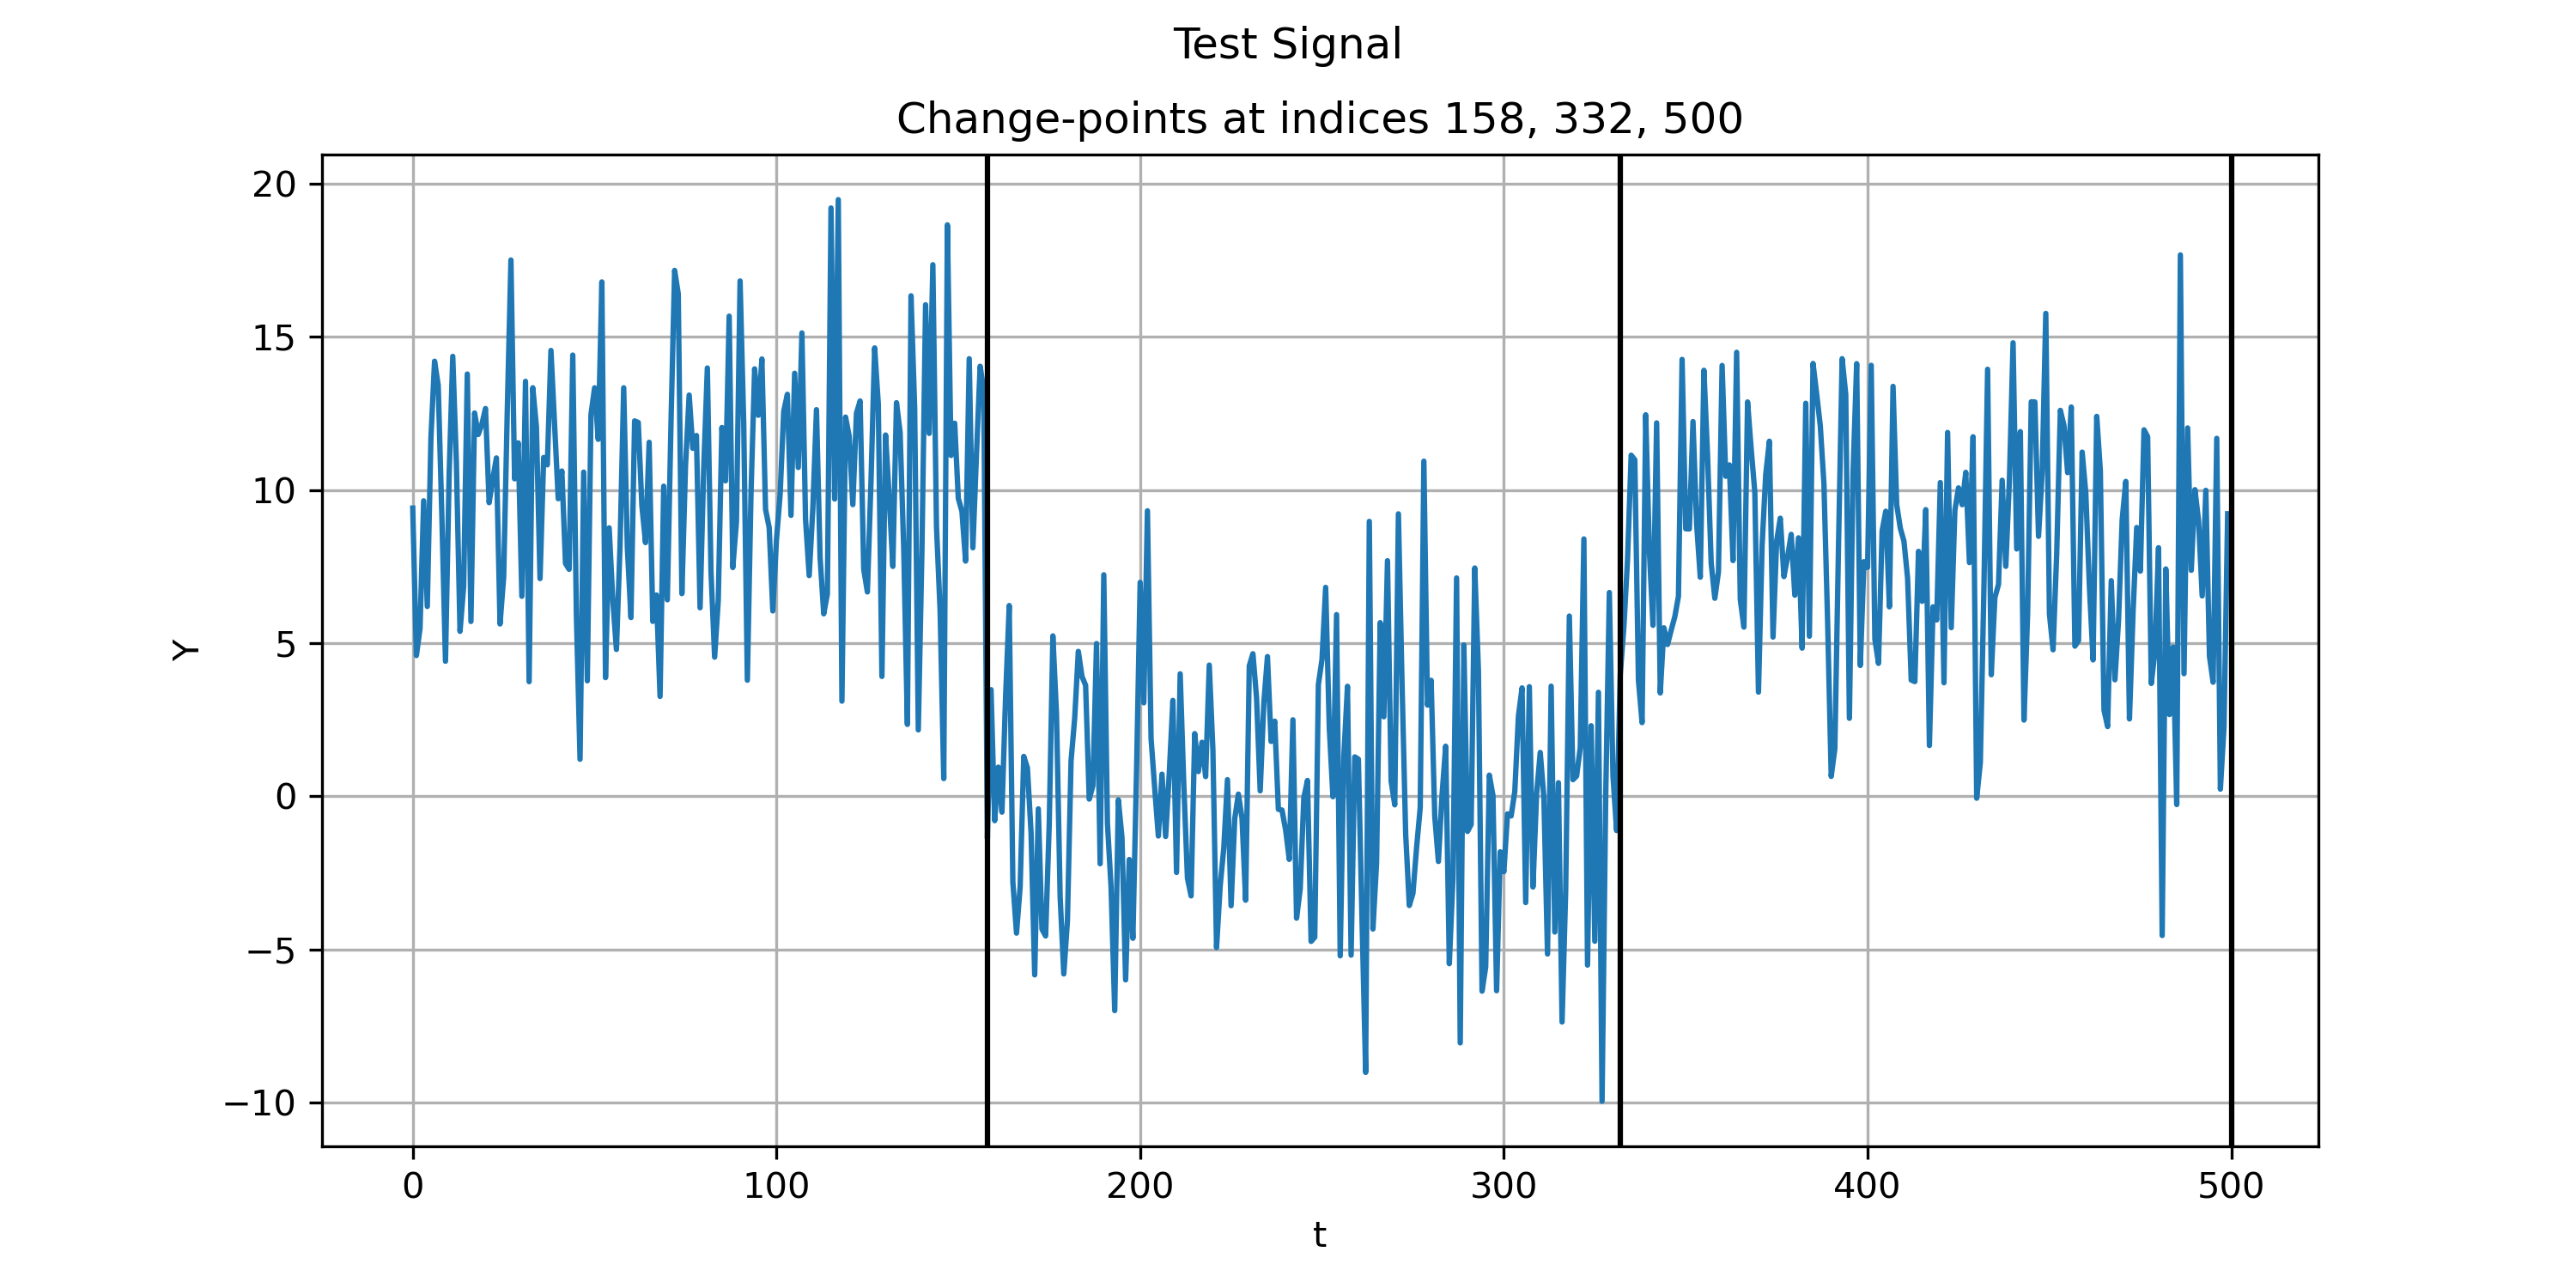
\includegraphics[scale=0.35]{show_series.png}
                    \caption{Piecewise constant signal with normal noise}
                    \footnote{The last index eases the software implementation}
                \end{figure}
            \end{frame}

            \begin{frame}{Search Algorithms}{Binary Segmentation}
                Greedy sequential algorithm that estimates 1st change-point as:
                \begin{equation}
                    \hat{t}_{1} := \argmin_{1 \leq t < T - 1} C(y_{0 \dots t}) + C(y_{t \dots T})
                \end{equation}

                It then repeats the operation on both left and right segments until the specified number of splits is achieved.

                \begin{figure}[!htbp]
                    \centering
                    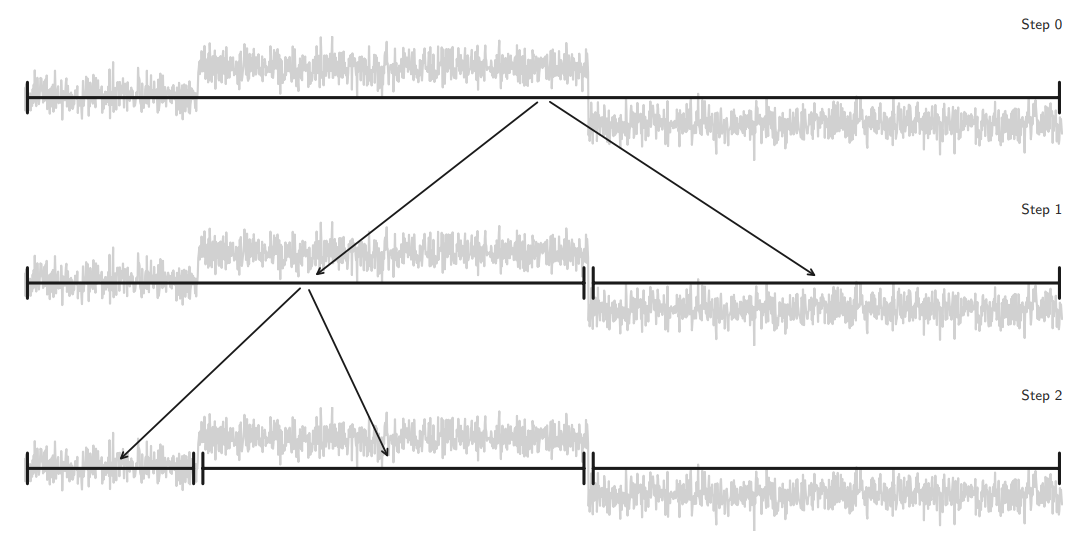
\includegraphics[scale=0.3]{bin_seg_schematics.png}
                    \caption{Overview of Binary Segmentation retrieved from \cite{truong2020selective}}
                \end{figure}
            \end{frame}

            \begin{frame}{Cost Functions}{L2 Norm}
                An estimator of shifts in the central point of a distribution. Given a series $\{y_t\}_{t \in \mathcal{I}}$ where  $y_t \in \mathbb{R}^d$:
                \begin{equation}
                    C(y_{\mathcal{I}}) = \sum_{d} \sum_{t \in \mathcal{I}} ||y_t - \bar{y} ||_{2}^{2}
                \end{equation}

                where $\bar{y}$ is the component wise mean of $y_{\mathcal{I}}$

                \begin{itemize}
                    \item Needs scaling, considering not to penalize on segment length
                \end{itemize}

            \end{frame}

            \begin{frame}{Feature Extraction}{Statistical Descriptors}
                Given a segment $S_{i}$ which encompasses $T_i$ timestamps, $S_i \in \mathcal{M}_{d}^{T_i}(\mathbb{R})$ with $T_i \geq \alpha$ where $\alpha$ is a constraint on the minimum size of $S_i$. We then use a set of descriptors $F_s = \{f \mid  f: \mathcal{M}_{d}^{T_i}(\mathbb{R}) \rightarrow \mathbb{R}^{d}\}$ as an example:
                \begin{table}[!htbp]
                    \begin{tabular}{ll}
                    \multicolumn{2}{c}{Statistical Descriptors} \\ \hline
                    Minimum & Std. Deviation \\
                    25th Percentile & Variance \\
                    Median & Kurtosis \\
                    75th percentile & Skew \\
                    Maximum & Coeff. of Variation \\
                    Mean & - \\ \hline
                    \end{tabular}
                \end{table}

                Applying each element of $F_s$ results on $S_i$ results in a feature vector $\hat{S}_i \in \mathbb{R}^{d \cdot |F_s|}$
            \end{frame}

            \begin{frame}{Data Reduction}

                A flight $F_i \in \mathcal{M}_{d}^{T_i}(\mathbb{R})$ contains $d \cdot T_i$ elements, the feature vector $\hat{F}_i \in \mathbb{R}^{d |F_s| \tau}$ contains $ d |F_s| \tau$ elements, where $|F_s|$ is the number of statistical descriptors used and $\tau$ is the number of segments chosen.

                As an example, use a flight with 5,000 timestamps, 10 features, 10 statistical descriptors and 4 segments:
                \begin{gather}
                    | F_i | = 10 \cdot 5,000 = 50,000 \\
                    | \hat{F}_i | = 10 \cdot 10 \cdot 4 = 400 \\
                    \frac{ | F_i | }{ | \hat{F}_i | } = 125 \label{eq:data-reduction}
                \end{gather}
            \end{frame}

            \begin{frame}{Methodology}{Pros \& Cons}
                \begin{columns}
                    \begin{column}{0.45\textwidth}
                        \begin{exampleblock}{Pros}
                            \begin{itemize}
                                \item Large data reduction, see \eqref{eq:data-reduction}
                                \item Lower computational load
                                \item Ease feature interpretation
                                \item Reproducible
                            \end{itemize}
                        \end{exampleblock}
                    \end{column}
                    \begin{column}{0.45\textwidth}
                        \begin{alertblock}{Cons}
                            \begin{itemize}
                                \item Mixed or uniform MVT segmentation?
                                \item Not a fixed number of stages in each flight
                                \item Which descriptors to use?
                            \end{itemize}
                        \end{alertblock}
                    \end{column}
                \end{columns}
            \end{frame}

        \subsection{RUL Prediction}

            \begin{frame}{RUL Prediction}{Interpretable ML models}
                Given the reduced dataset, one now must select a model to estimate RUL. But how can you choose without prior information?
                \begin{enumerate}
                    \item Define a common loss function
                    \item Apply data transformation techniques \footnote{Any transformation must also be interpretable}
                    \item Select a suite of \textbf{interpretable} ML models
                    \item Baseline testing (w/o tuning) and ranking
                    \item Candidate model selection
                    \item Repeat!
                \end{enumerate}
            \end{frame}

        \subsection{Model Interpretation}
            \begin{frame}{Model Interpretation}{Importance and Benefits}

                \begin{columns}
                    \begin{column}{0.5\textwidth}
                        Interpretability enables \textbf{transparency} and \textbf{accountability}
                        \begin{itemize}
                            \item Analyze the weights of each feature in linear regression
                            \item Check the splits in a decision tree
                            \item Marginal changes in features affecting log-odds for logistic regression
                            \item Shapley and LIME for \enquote{higher models}
                        \end{itemize}
                    \end{column}
                    \begin{column}{0.5\textwidth}
                        \begin{figure}[!htbp]
                            \centering
                            \includegraphics[scale=0.15]{amazon_sexist.png}
                            \caption{Amazon removes its recruitment algorithm due to gender bias towards men \cite{reporter-2018}}
                        \end{figure}
                    \end{column}
                \end{columns}
            \end{frame}

        \begin{frame}{Model Interpretation}{Properties of Shapley values}

            \begin{itemize}
                \item \textbf{Efficiency:}\begin{equation*}
                    \sum_{j=1}^{p} \phi_j = \hat{f}(x) - \mathbb{E}[\hat{f}(X)]
                \end{equation*}
                \item \textbf{Symmetry:} \begin{equation*}
                    \begin{split}
                        val(S \cup \{j\}) & = val(S \cup \{k\}) \quad \forall S \subseteq \{1, \dots, p\} - \{j, k\} \\
                        & \Rightarrow \phi_j = \phi_k
                    \end{split}
                \end{equation*}
                \item \textbf{Dummy:}  \begin{equation*}
                    \begin{split}
                        val(S \cup \{j\}) & = val(S) \quad \forall S \subseteq \{1, \dots, p\} \\
                        & \Rightarrow \phi_j = 0
                    \end{split}
                \end{equation*}
                \item \textbf{Additivity:} \begin{equation*}
                    \phi_j^{f + g} = \phi_j^{f} + \phi_j^{g}
                \end{equation*}
            \end{itemize}
        \end{frame}

        % \begin{frame}{Model Interpretation}{Analyzing Principal Components}
        %     \begin{algorithm}[H]
        %         \begin{algorithmic}[1]
        %             \STATE $x_s \leftarrow X[s]$ \COMMENT{Sample from raw dataset}
        %             \STATE $E_f \leftarrow P[f]$ \COMMENT{Subset of explanatory features}
        %             \STATE $\epsilon \leftarrow 0.1$ \COMMENT{Error treshold}
        %             \STATE $F_w \leftarrow E$ \COMMENT{PCA component's matrix}
        %             \FOR{$f$ in $E_f$}
        %                 \STATE $x_p \leftarrow X_p[s, f]$
        %                 \STATE $w_{idx} \leftarrow argsort(abs(F_w[:, f]))$
        %                 \STATE $approx \leftarrow cumsum(x_s[w_{idx}] * F_w[w_{idx}, f])$
        %                 \STATE $f_i \leftarrow argmax (abs(approx / x_p)) \geq 1 - \epsilon $
        %                 \STATE $\Hat{x}_p \leftarrow x_s[w_{idx}][:f_i] \cdot F_w[w_{idx}, f][:f_i]$
        %                 \PRINT $x_s[f_i], x_p, \Hat{x}_p, F_w[f_i]$
        %             \ENDFOR
        %         \end{algorithmic}
        %         \caption{Pseudocode for the calculation of truncated explanations}
        %         \label{alg:seq}
        %     \end{algorithm}
        % \end{frame}

        % \begin{frame}{Model Interpretation}{An example of truncated explanations}
        %     Given a dataset $X \in \mathcal{M}_{100}^{5}(\mathbb{R})$, a target feature $y \in \mathbb{R}$. PCA is applied on $X$ to get $X_{proj}$ and $W$, a model $\hat{f}$ is trained on $X_{proj}$ to predict $y$. We're interested on sample $x_s$ and know $PC0, PC3$ contributed the most to its corresponding estimate. Checking $PC0$:
        %     \begin{gather*}
        %         x_s = [0.843, 0.069, 0.894, 0.089, 0.163] \\
        %         X_{std} = [0.975, 0.012, 0.869, -0.022, 0.291] \\
        %         w =  [0.450, -0.343,  0.510,  0.638, -0.100] \\
        %         x_{proj} = 0.835 \\
        %         w_{idx} = [3, 2, 0, 1, 4] \\
        %         approxs = [-0.0146,  0.4292,  0.8689,  0.8644,  0.8351] \\
        %         selected = [3, 2, 0]
        %     \end{gather*}
        % \end{frame}

        \subsection{Prediction Intervals}

            \begin{frame}{Prediction Intervals}{Estimating uncertainty}

                \begin{columns}
                    \begin{column}{0.5\textwidth}
                        All predictions have an inherent level of uncertainty. \enquote{A prediction interval provides an estimate range within which a future observation is likely to fall} \cite{peters-2023}
                        \begin{exampleblock}{Machine Learning Perspective}
                            In ML, they represent the range within which a predicted observation is likely to fall, they estimate the uncertainty of point estimates.
                        \end{exampleblock}
                    \end{column}
                    \begin{column}{0.5\textwidth}
                        \begin{figure}[!htbp]
                            \centering
                            \includegraphics[scale=0.4]{sample_confidence_vs_prediction.png}
                            \caption{Difference between CIs and PIs \cite{cialdella-2020}}
                        \end{figure}
                    \end{column}
                \end{columns}
            \end{frame}

            \begin{frame}{Prediction Intervals}{Quantile Regression}

                Let $\tau$ be the selected quantile, $y$ the target variable and $\hat{y}$ the predicted quantile. The \textbf{Pinball Loss} is defined as:
                \begin{equation}\label{eqn:pinball}
                    \mathcal{L}_\tau(y, \hat{y}) = (y - \hat{y}) \tau \mathds{1} \left\{y \geq \hat{y}\right\} + (\hat{y} - y) (1 - \tau) \mathds{1} \left\{\hat{y} > y\right\}
                \end{equation}

                \begin{equation}\label{eqn:koenker_min}
                    \mathcal{Q}_\tau(Y | X) = \argmin_{q(X)} \mathbb{E}[\mathcal{L}_\tau(Y, q(X))]
                \end{equation}

                Koenker introduced the concept of quantile regression in 1978, and continued its development up to the Conditional Quantile Functions \cite{koenker2001quantile} referenced in \eqref{eqn:koenker_min} which minimizes \eqref{eqn:pinball}
            \end{frame}

        \subsection{Hyperparameter Optimization}

            \begin{frame}{Hyperparameter Optimization}{Overview}
                \begin{columns}
                    \begin{column}{0.5\textwidth}
                        Each dataset and model is different, and there is no rigorous proof on how to determine the optimal hyperparameters for a given problem. We adopt approximated methods divided into 3 categories \cite{aws-hyperparameter}:
                        \begin{itemize}
                            \item Grid Search
                            \item Random Search
                            \item \textbf{Bayesian Optimization}
                        \end{itemize}
                    \end{column}
                    \begin{column}{0.5\textwidth}
                        \begin{figure}[!htbp]
                            \centering
                            \includegraphics[scale=0.35]{hyperparameter_search.png}
                        \end{figure}
                    \end{column}
                \end{columns}
            \end{frame}

            \begin{frame}{Hyperparameter Optimization}{Tree-structured Parzen Estimators}

                Given a search history, it suggests a hyperparameter for the next trial.
                \begin{itemize}
                    \item Treats each hyperparameter \textbf{independently}
                    \item Processes search history as tuples of (parameter, loss)
                    \item Updates the definition of \enquote{good} and \enquote{bad} losses
                    \item Defines $g(x)$ and $b(x)$ for good and bad losses
                \end{itemize}

                \begin{exampleblock}{Heuristic}
                    Select the hyperparameter which maximices:
                    \begin{equation}
                        x_s = \argmax_{x} \frac{g(x)}{b(x)}
                    \end{equation}
                \end{exampleblock}
            \end{frame}

            \begin{frame}{Hyperparameter Optimization}{Tree-structured Parzen Estimators Overview}
                \begin{figure}[placement]
                    \centering
                    \includegraphics[scale=0.8]{bayesian_algo_overview.png}
                    \caption{Example of TPE trial suggestion \cite{pmlr-v139-tiao21a}}
                \end{figure}
            \end{frame}

    \section{Experimental Results}

        \begin{frame}{Segmentation of Environmental Descriptors}
            For a test case we apply Binary Segmentation with L2 norm and min. size for segment of 20\% the length of the array
            \begin{figure}
                \centering
                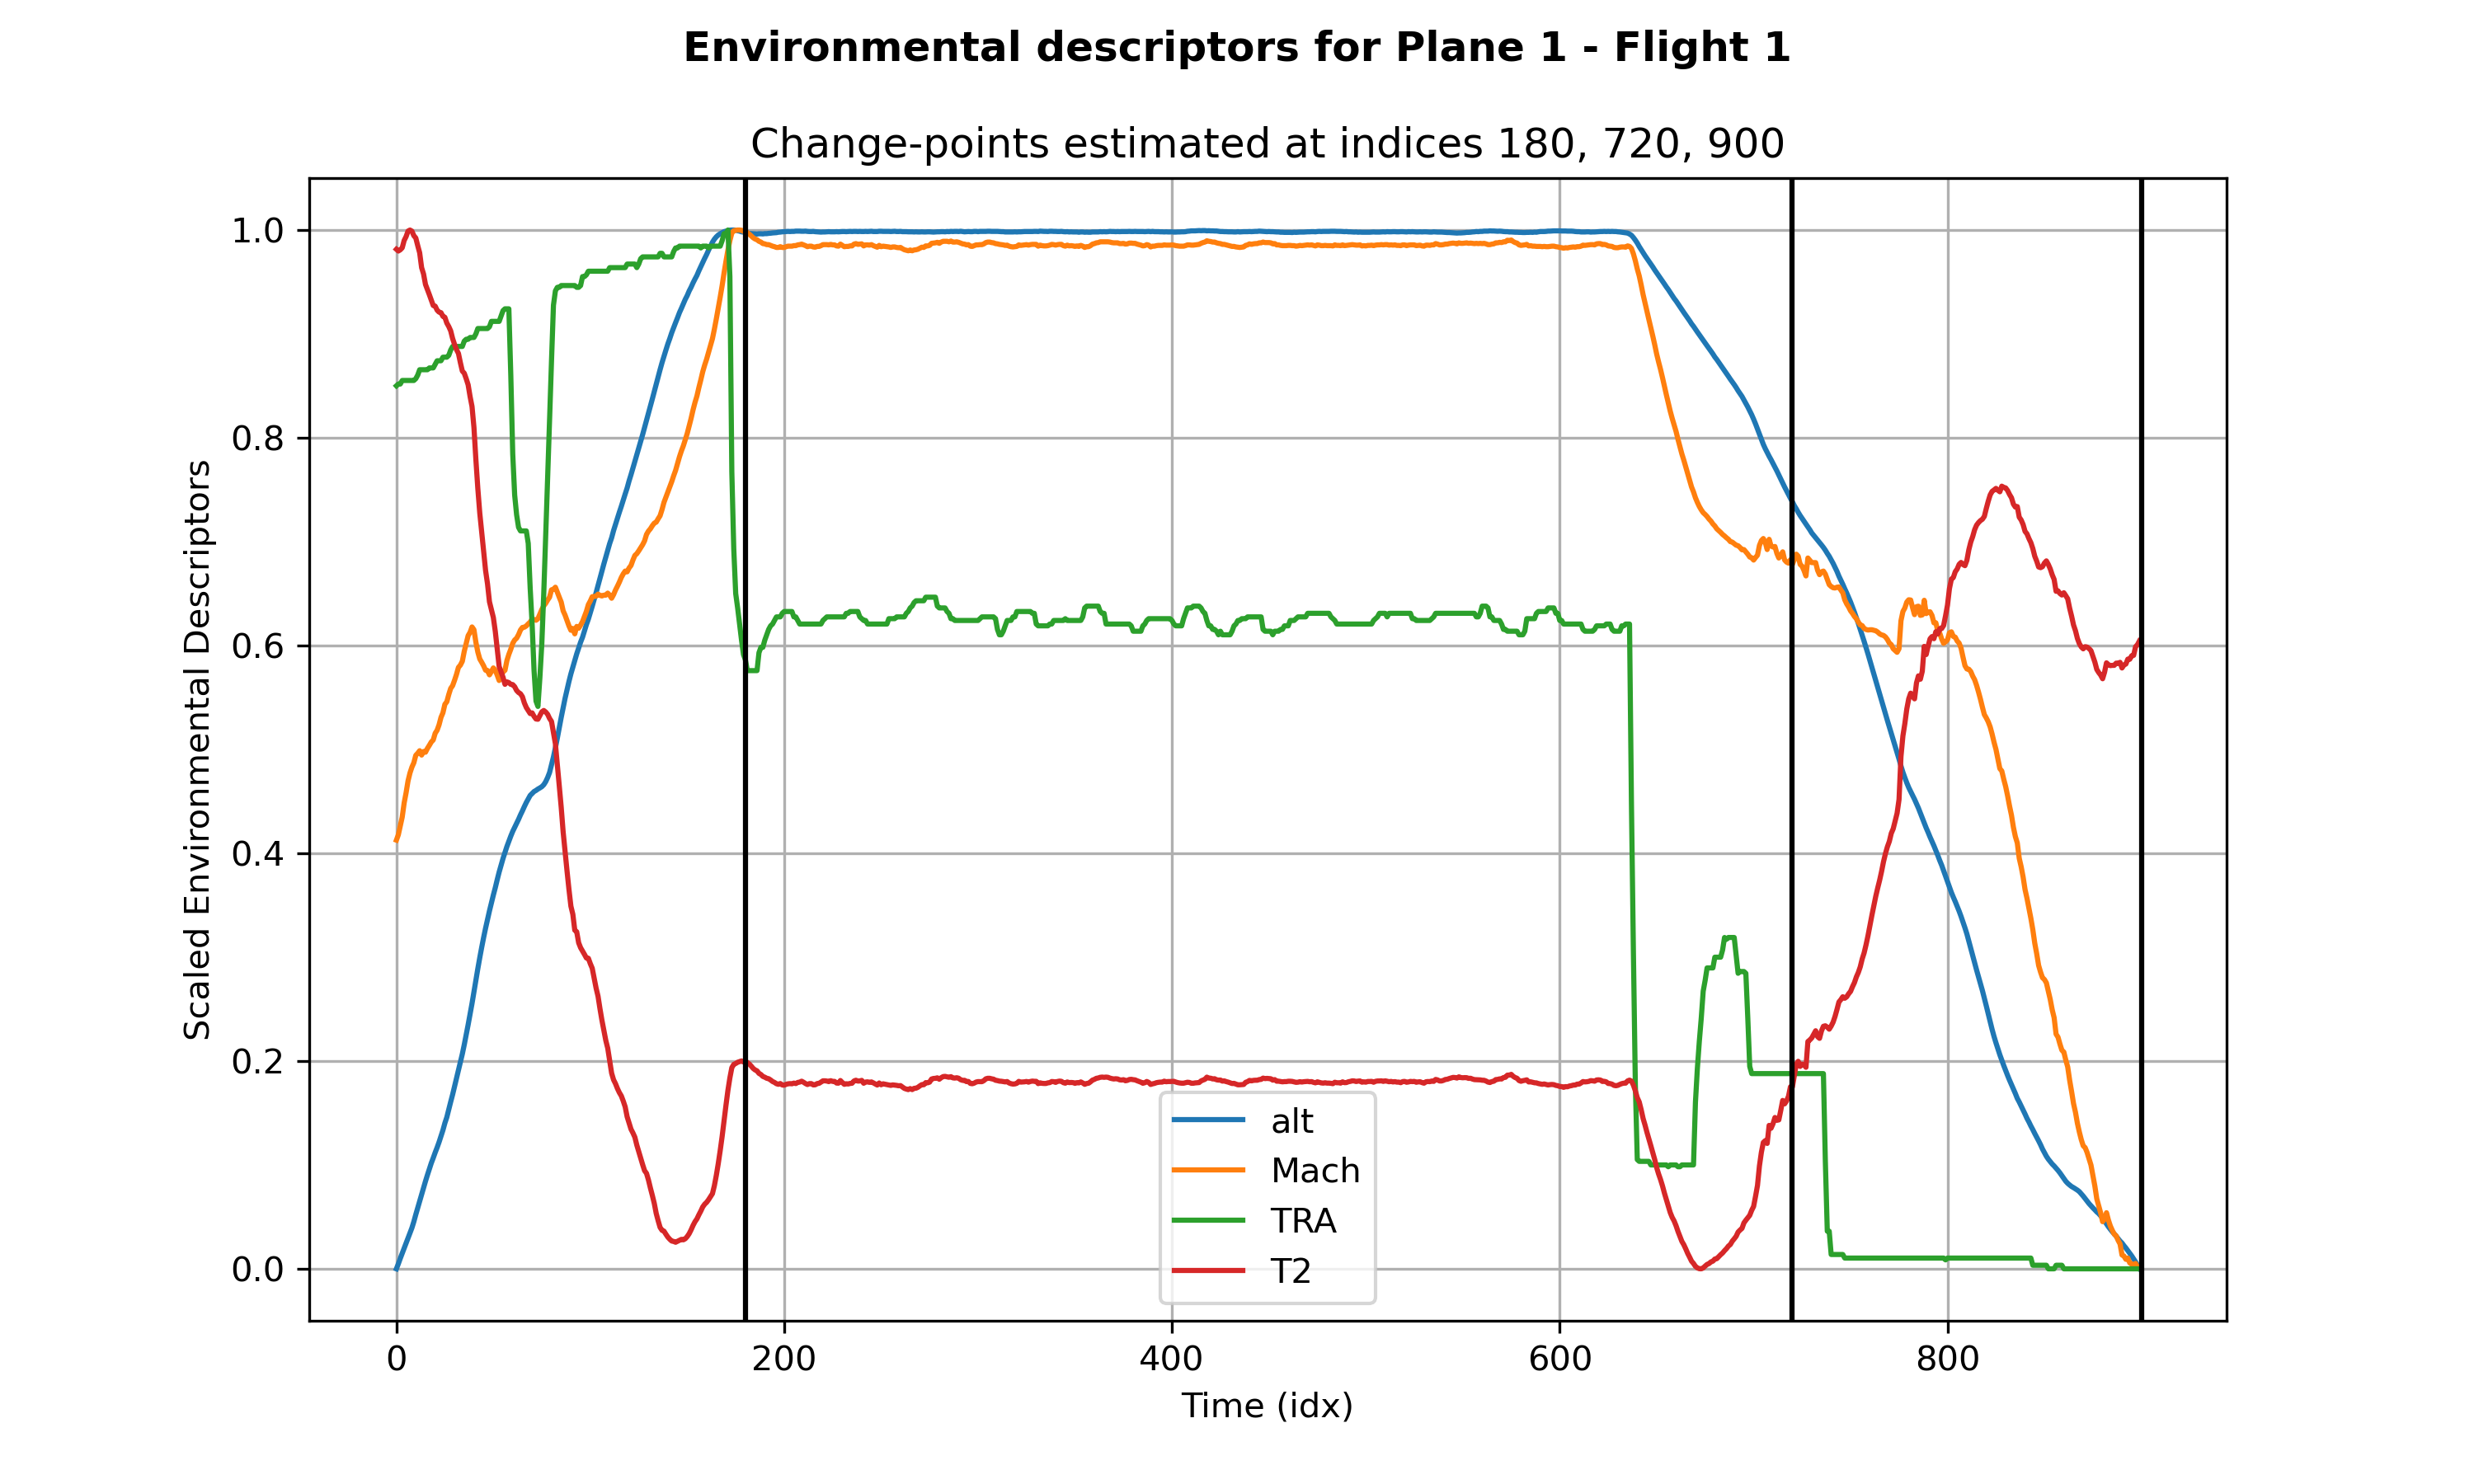
\includegraphics[scale=0.35]{environment_split_1_1.png}
                \caption{Environmental descriptors (scaled) for the first flight for plane 1}
            \end{figure}
        \end{frame}

        \begin{frame}{Flight History of a Plane}
            \begin{figure}
                \centering
                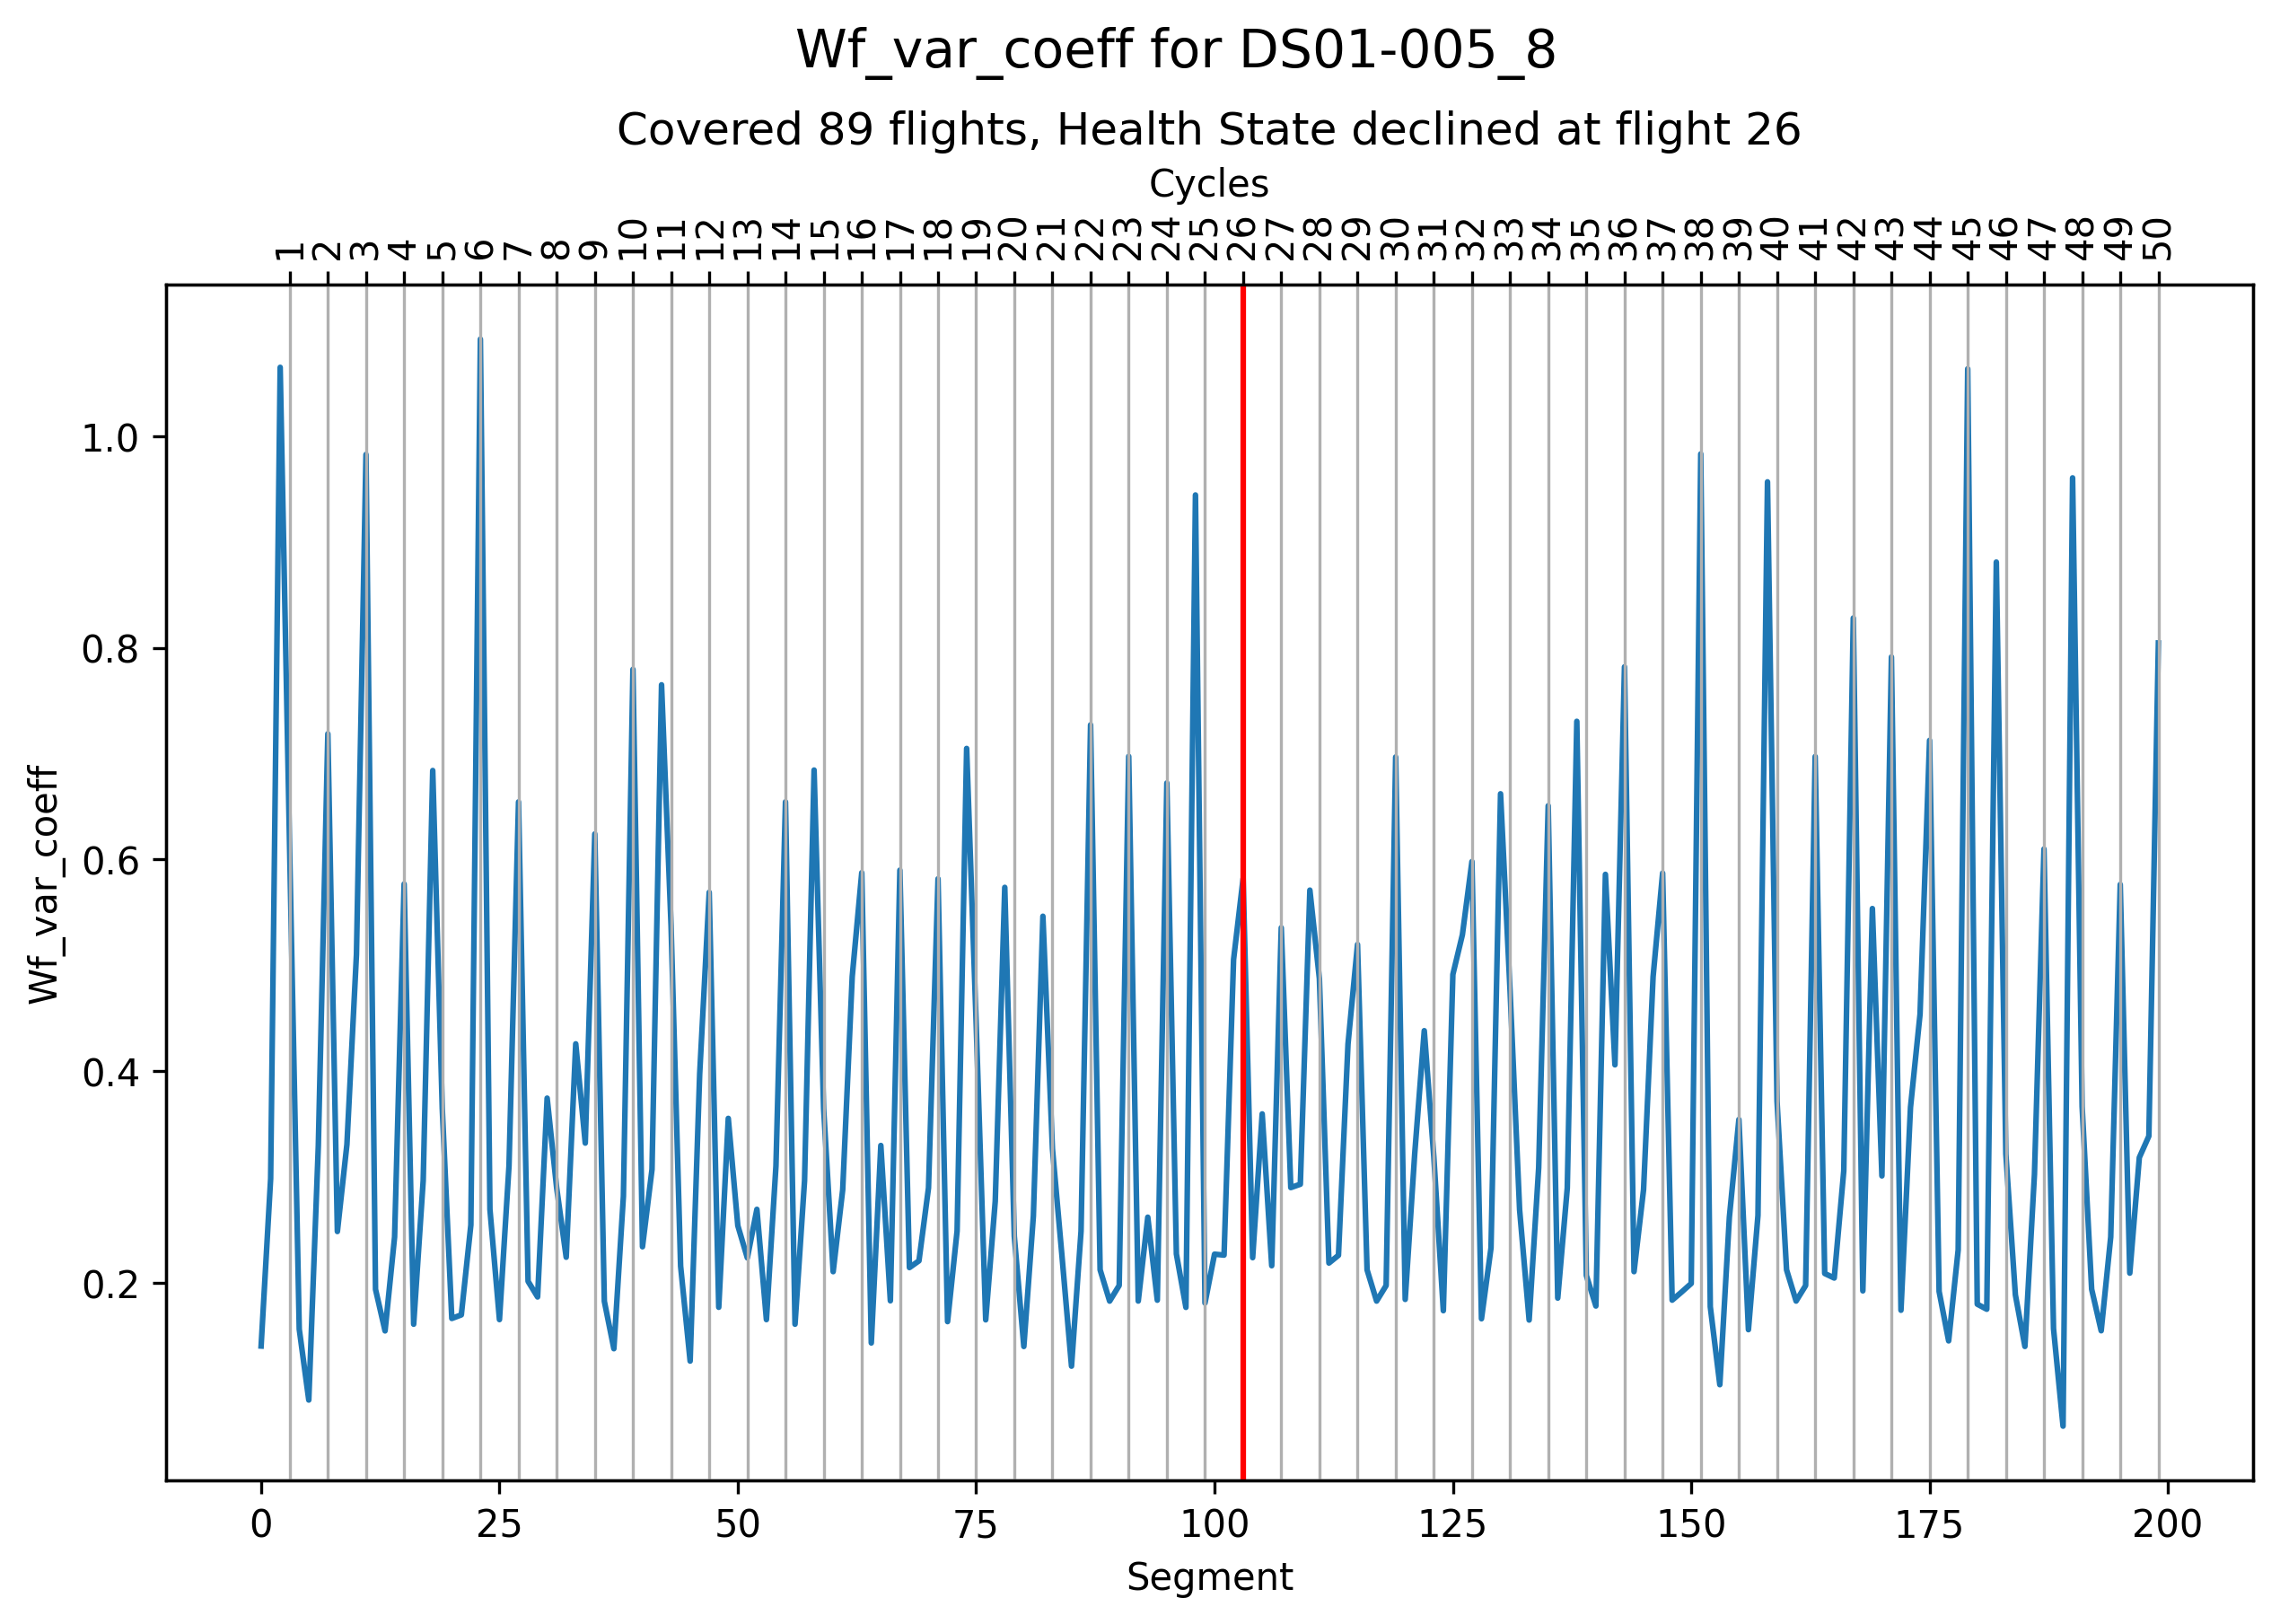
\includegraphics[scale=0.35]{DS01-005_8_Wf_var_coeff.png}
                \caption{Coefficient of variation of the Fuel Flow for Unit 8. Flew 89 flights}
            \end{figure}
            Could there be a correlation between the early spikes and the relatively early health decline?
        \end{frame}

        \begin{frame}{Baseline Regression Models}

            A suite of interpretable ML models is fit to 80\% of the resulting dataset, tested on the remaining 20\%
            \begin{table}[!htbp]
                \scalebox{0.6}{
                \begin{tabular}{llllllll}
                \hline
                Model & Train Loss & Test Loss & Train R2 & Test R2 & Train RMSE & Test RMSE & Fit Time \\
                \hline
                Catboost & 4.925814 & 6.81856 & 0.888255 & 0.793759 & 7.918826 & 11.036592 & 30.923586 \\
                XGBoost & 3.992694 & 6.902025 & 0.928544 & 0.78922 & 6.332358 & 11.157376 & 6.510977 \\
                \textbf{LGBM} & \textbf{4.861673} & \textbf{6.983948} & \textbf{0.891184} & \textbf{0.784365}  & \textbf{7.81434} & \textbf{11.285139} & \textbf{2.113664}  \\
                Random Forest & 2.824662 & 7.209788 & 0.967582 & 0.77276 & 4.265207 & 11.584841 & 216.538052 \\
                Ridge & 6.840865 & 7.275478 & 0.783071 & 0.766391 & 11.033299 & 11.746066 & 0.05542 \\
                Lasso Lars & 7.30732 & 7.420427 & 0.753777 & 0.75725 & 11.754672 & 11.973661 & 0.064927 \\
                Lasso & 7.307333 & 7.420434 & 0.753776 & 0.75725 & 11.754695 & 11.973673 & 0.122003 \\
                Elastic Net & 7.363291 & 7.47165 & 0.750416 & 0.754214 & 11.834634 & 12.048292 & 0.237217 \\
                SVM & 7.36937 & 7.60994 & 0.748435 & 0.744574 & 11.881503 & 12.282309 & 13.777651 \\
                Decision Tree & 0.5 & 9.758508 & 1.0 & 0.625179 & 0.0 & 14.878505 & 3.323056 \\
                Dummy (Mean) & 17.27968 & 17.824815 & 0.0 & -0.004084 & 23.688969 & 24.351877 & 0.002806 \\
                Linear Regression & 5.642092 & 87743.731314 & 0.852029 & 0.635906 & 9.112421 & 14.664064 & 0.257621 \\
                \hline
                \end{tabular}
                }
            \end{table}

            \begin{enumerate}
                \item LGBM achieves similar accuracy as Catboost and XGBoost but in a fraction of their training time
                \item Linear models present less overfitting but comparatively lower accuracy
            \end{enumerate}
        \end{frame}

        \begin{frame}{Dimensionality Reduction?}
            PCA on raw descriptors needs 28 components to explain 99\% of the total variance:
            \begin{figure}
                \centering
                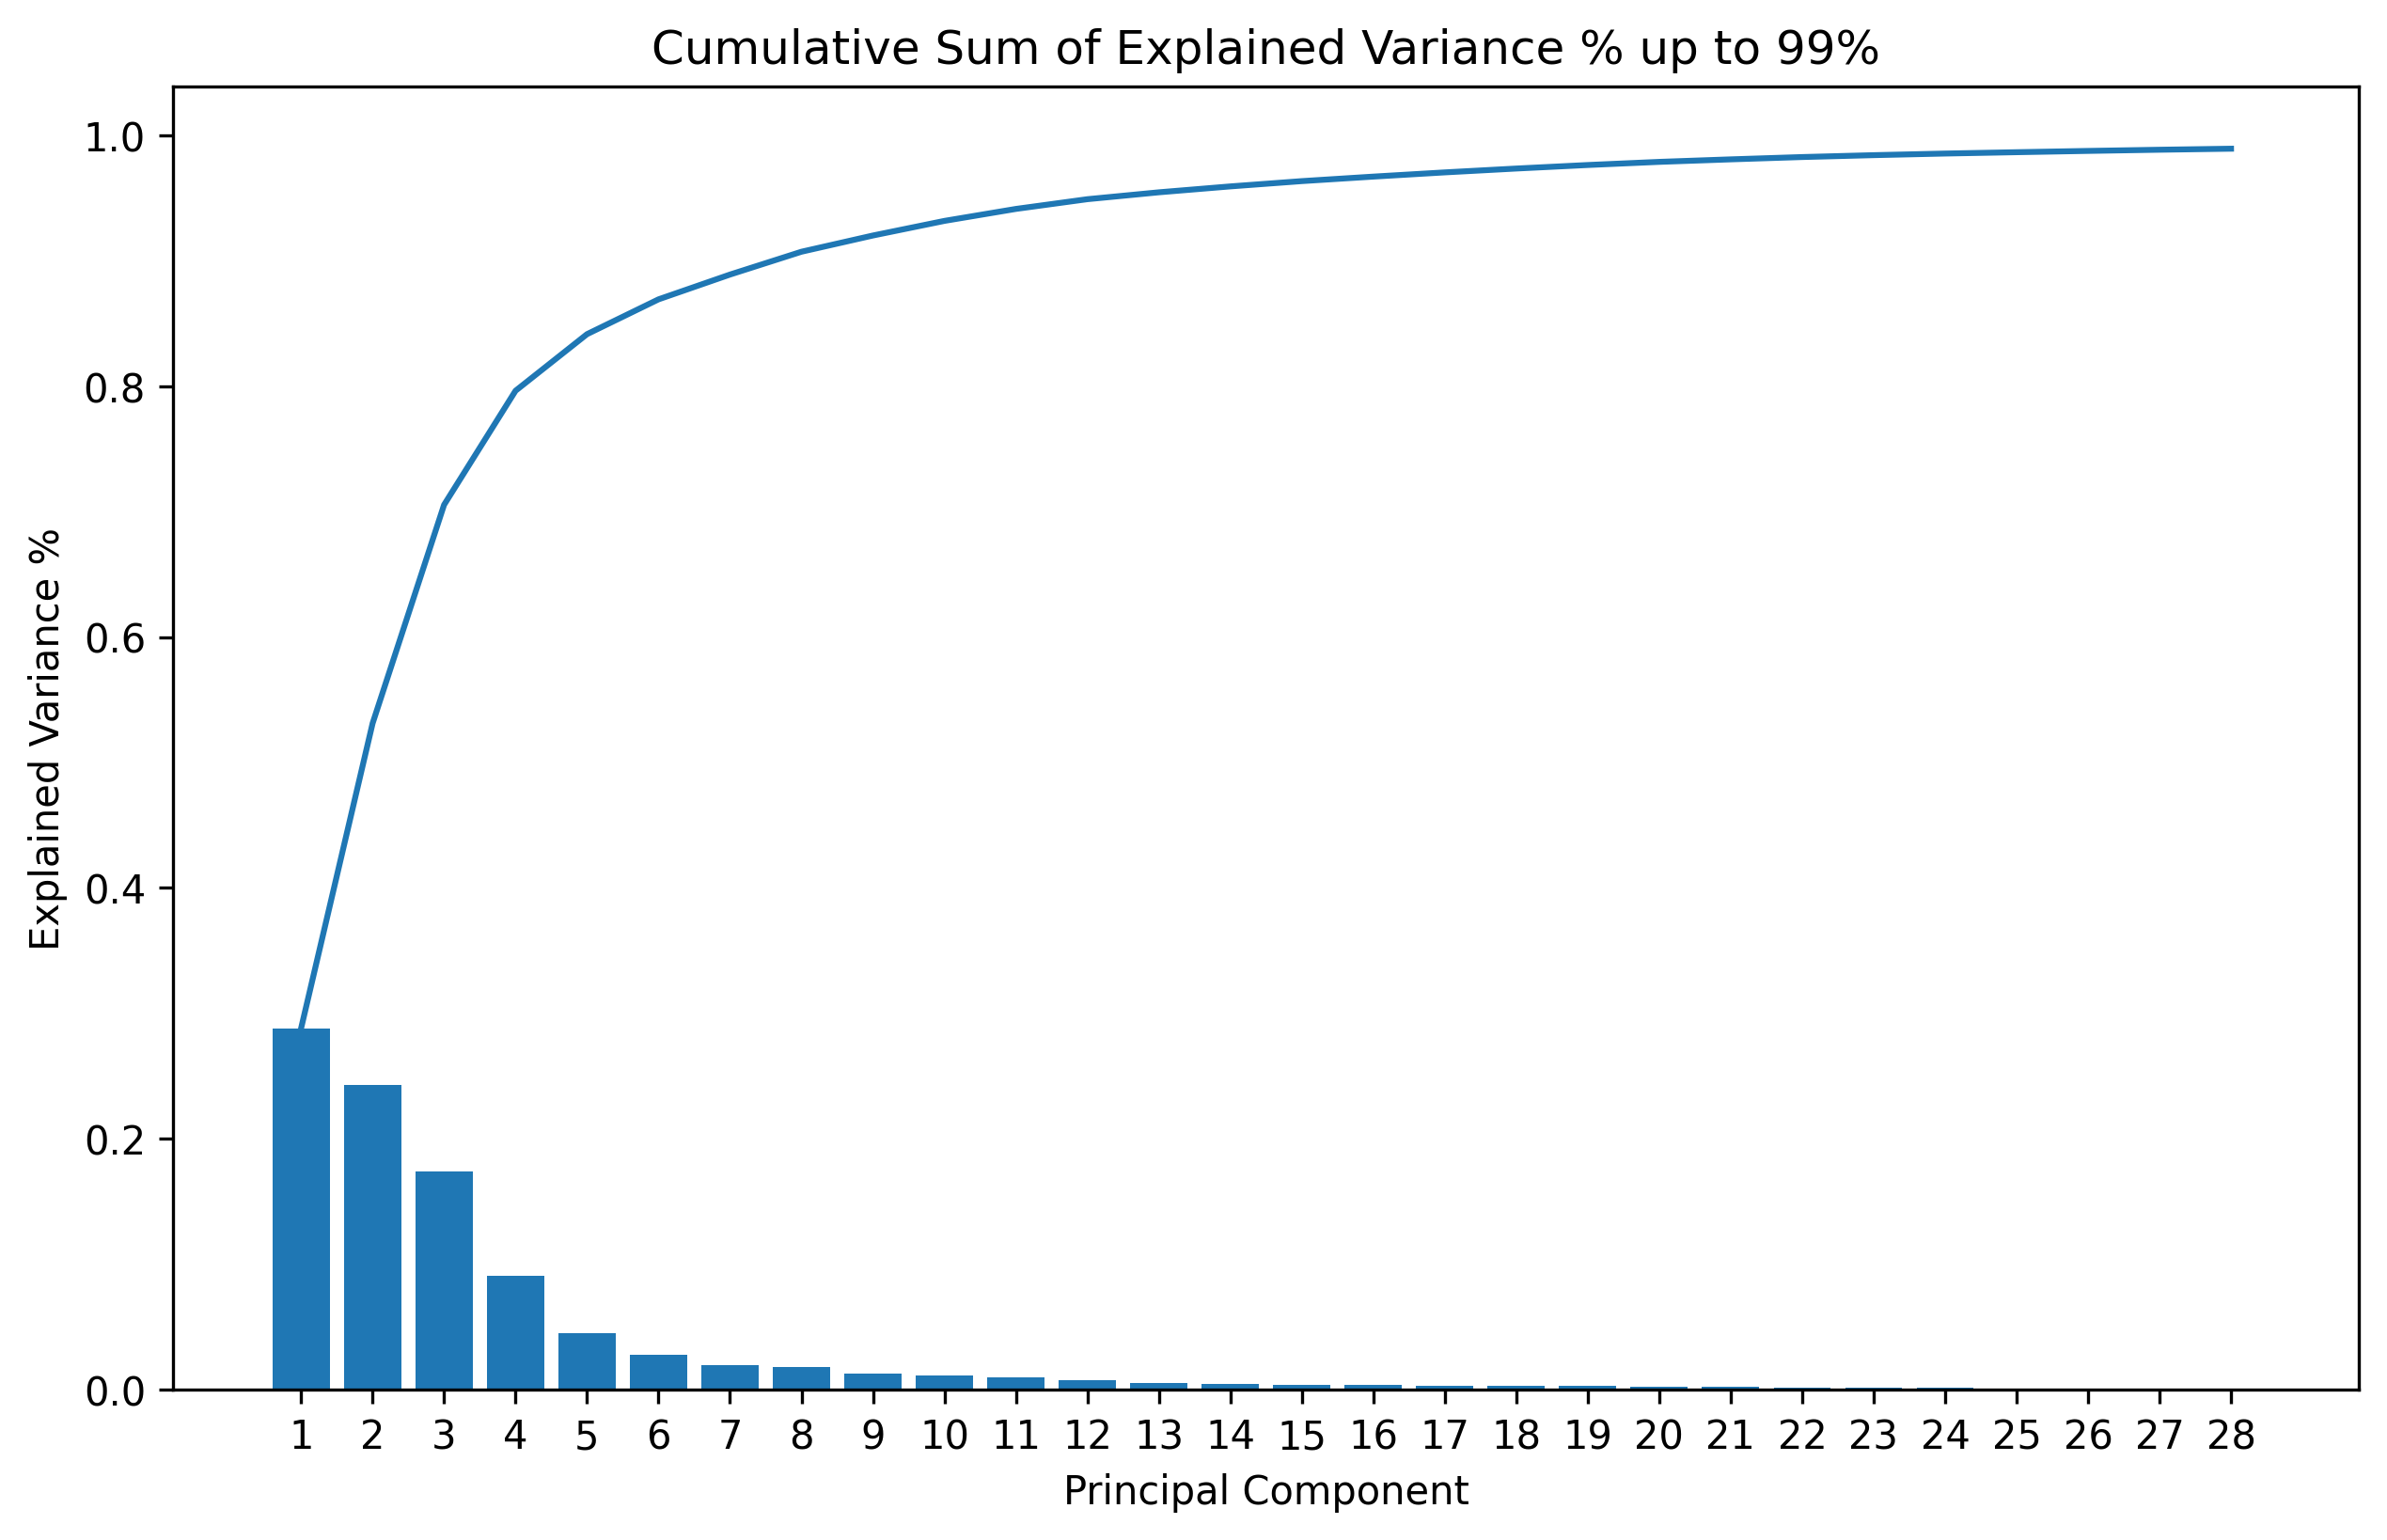
\includegraphics[scale=0.35]{pca_99_untransformed.png}
                \caption{Explained variance ratio per Principal Component added up to 99\%}
            \end{figure}

            \textbf{Scaled PCA needs 93}, nonetheless weights should be distributed fairly, doesn't imply better prediction performance!
        \end{frame}

        \begin{frame}{Effects on Model Accuracy subject to prior Standarization}

            Using a LGBM regressor as a baseline model, the following treatments were tested on a validation dataset:
            \begin{table}[!htbp]
                \begin{tabular}{ll}
                    \hline
                    Transformation & Test Loss \\
                    \hline
                    No PCA & 6.983 \\
                    Raw, all PCs & 5.867 \\
                    Raw, 28 PCs & 7.229 \\
                    Standardized, all PCs & 6.786 \\
                    Standardized, 93 PCs & 7.506 \\
                    \hline
                \end{tabular}
            \end{table}

            PCA enables an overall improvement on model loss, but the model doesn't rely on the \textit{most} important components.
        \end{frame}

        \begin{frame}{Sample Predictions}
            Using a basic LGBM model with 100 epochs yields:
            \begin{figure}
                \centering
                \includegraphics[scale=0.35]{lgbm_preds_DS01-005_7.png}
                \caption{RUL estimates and deviations from real RUL for plane 7 of dataset DS01-005}
            \end{figure}
        \end{frame}

        \begin{frame}{Sample Predictions}
            \begin{figure}
                \centering
                \includegraphics[scale=0.35]{lgbm_preds_DS02-006_15.png}
                \caption{RUL estimates and deviations from real RUL for plane 15 of dataset DS02-006}
            \end{figure}
        \end{frame}

        \begin{frame}{Model interpretation}

            Next we show the overall importance of each Principal Component in RUL regression:
            \begin{figure}
                \centering
                \includegraphics[scale=0.35]{global_shap_importance.png}
                \caption{SHAP values for the Top 7 features (selected by the mean absolute value across all predictions)}
            \end{figure}

            The first 3 Principal Components appear in the Top 7, but are not the most important
        \end{frame}

        \begin{frame}{Instance Explanation}

            We can also analyze in detail a single RUL estimate:
            \begin{figure}
                \centering
                \includegraphics[scale=0.35]{flight_sample_explanations.png}
                \caption{SHAP values for the Top 7 features (selected by the mean absolute value across all predictions)}
            \end{figure}
        \end{frame}

        \begin{frame}{Example of estimated prediction intervals}
            Fitting a base LGBM for RUL estimates and 2 models for quantile regression using pinball loss:
            \begin{figure}
                \centering
                \includegraphics[scale=0.5]{test_intervals.png}
                \caption{RUL estimates and a 90\% prediction interval for a plane}
            \end{figure}
        \end{frame}

        \begin{frame}{TPE Hyperparameter Optimization}
            Defined a common search space with hyperparameters available for XGBoost Regressors. The optimization regime constrained is to 1500 iterations per model, for the following search space:

            \begin{table}[!htbp]
                \centering
                \scalebox{0.7}{
                \begin{tabular}{ll}
                    \hline
                    Parameter & Range \\
                    \hline
                    Learning Rate & $\exp (\mathcal{U}(-10, 0))$ \\
                    Boosting Rounds & $\mathcal{U}(100, 10000)$ \\
                    Max Depth & $\mathcal{U}(2, 25)$ \\
                    Min Child Weight & $\mathcal{U}(2, 50)$ \\
                    Subsample & $\mathcal{U}(0.2, 1)$ \\
                    Subsample by Tree & $\mathcal{U}(0.2, 1)$ \\
                    Subsample by Node & $\mathcal{U}(0.2, 1)$ \\
                    Subsample by Level & $\mathcal{U}(0.2, 1)$ \\
                    Gamma & $ \exp (\mathcal{U}(-10, 10))$ \\
                    Alpha & $ \exp (\mathcal{U}(-10, 10))$ \\
                    Lambda & $ \exp (\mathcal{U}(-10, 10))$ \\
                    \hline
                \end{tabular}}
            \end{table}

            \textbf{TPE optimizes the mean cross-validated PHMAP test loss across 5 folds}

        \end{frame}

    \section{Conclusions}

    \section*{References}
        \begin{frame}[allowframebreaks]
            \frametitle{References}
            \printbibliography
        \end{frame}
\end{document}
